\chapter{Results}

\begin{table}[!t]
	\begin{tabular}{|>{\centering}p{2.5cm}|>{\centering}p{2.5cm}|>{\centering}p{2.5cm}|>{\centering}p{2.5cm}|>{\centering}p{2.5cm}|}
		\hline 
		number of processed routes & dummy atoms (mean) & atoms/dummy region (mean) & number of cycles (mean) & polycyclic {[}\%{]}\tabularnewline
		\hline 
		378 & 26.97 & 16.30 & 1.66 & 30.16\tabularnewline
		\hline 
	
	\end{tabular}\caption{Some statistics about the twenty ligands selected from the PDBbind-CN database and the calculations they were used for. Number of processed routes: total number of computed routes for a specific combination of two molecules; dummy atoms (mean): average number of total dummy atoms required for the computed mutation routes; atoms/dummy region (mean): number of total dummy atoms divided by the number of dummy regions; number of cycles (mean): average number of cyclic structural elements in all mutation routes; polycyclic: percentage of mutation routes which involve polycyclic structures, i.e., there are atoms present that participate in multiple cyclic elements }
\label{tab:general_information}
\end{table}

A set of twenty ligands from the PDBbind-CN database were downloaded and used for testing
CC construction, as well as mutation routes. General information about the ligands can be found in table \ref{tab:general_information}. 
It should be noted, however, that the CCs for some of these ligand pairs
violate the rules of {\trafo} concerning a valid CC; i.e., dummy regions are connected by more
than one atom to the CC (which basically implies that the
atom is part of a ring structure). 

In the current implementation of the mutation algorithm, this problem
is solved by a helper function which chooses one of the possible connections
between one of the atoms to the CC. For the following processing
of the mutation algorithm, this connection is arbitrarily distinguished
and the other ones removed. 


\section{Visualizations}

The mutation route is visualized using a color gradient, in addition
to numbering, see the earlier figures.
Py3dMol \cite{key-4} is used for a 3D-animation of the mutation process. Fig. \ref{fig:py3dmol} shows two molecules and their shared CC.

\begin{figure}
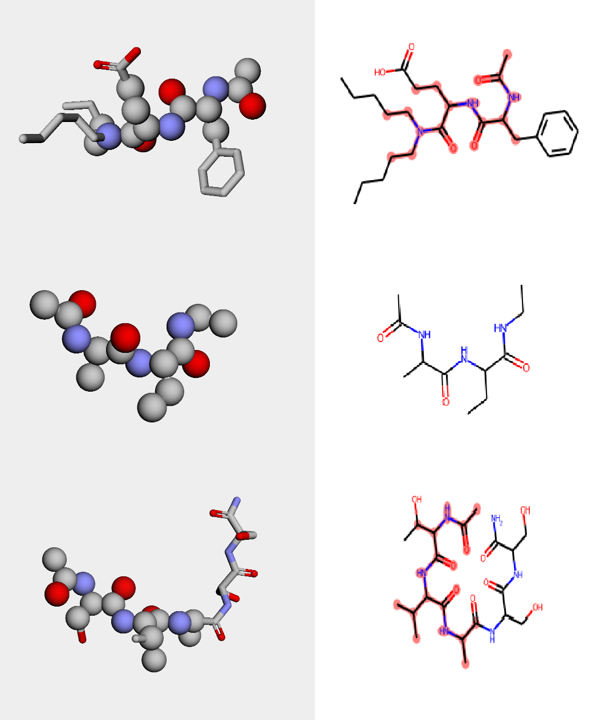
\includegraphics[scale=0.95]{trafo_py3d_2}

\caption{Two Visualizations of the mutation route with Py3Dmol (left column) and RDKit (right column). First and third row: Representation of the physical end states, left: spheres represent CC atoms, whereas non-CC atoms are shown in licorice representation; right: CC atoms are highlighted in red. Middle row: CC of the two end states.
}
\label{fig:py3dmol}
\end{figure}


\section{Scoring schemes}

Several scoring schemes have been implemented to assess and compare
the mutation routes proposed by the new algorithms.\\
1) Betweenness centrality: Betweenness centrality measures the number
of shortest paths going through a specific node \cite{Newman.2010}. More central atoms
will have a higher, atoms remote from
the CC will have a lower centrality coefficient. In particular, the last atom of a chain
has a coefficient of 0 because no path between two other atoms visits
the representing node. After each step, the node is removed from
the graph.
For avoiding undesired mutations, the maximum betweenness centrality
of all mutation steps is more decisive; hence, the average of the mean
as well as the maximum betweenness centrality of all removed nodes
is shown below.

\begin{figure}[H]
	
	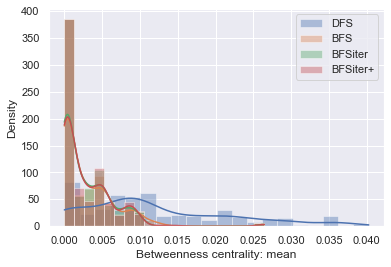
\includegraphics[scale=0.8]{betweenness_mean_all}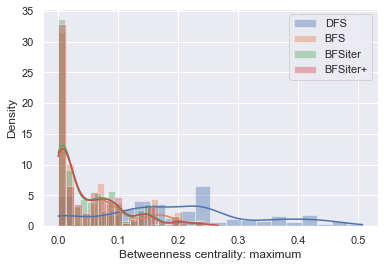
\includegraphics[scale=0.8]{betweenness_max_all}\caption{Betweenness centrality for the test ligands from the PDBbind-CN data set. Maximum and mean betweenness centrality are much higher for DFS than for all BFS-based mutation route algorithms. Curves are density estimates of the histograms.}
	\label{fig:betweenness_centrality}
\end{figure}

2) Closeness centrality: Closeness centrality of a specific node is
given by the inverted distances between this node and all other nodes
of the graph \cite{Newman.2010}. Similar to betweenness centrality, more 'important', central atoms have a higher closeness centrality, whereas atoms more distant from the CC have a lower
closeness centrality.
For using this centrality measure as a scoring function for the mutation
algorithms, the dummy region with the highest number of atoms (simply
because this is probably the most \textquoteleft interesting\textquoteright{}
one, it would also be possible to take the average of all dummy regions
etc.) is selected. The closeness centrality of each node representing a dummy atom for
the full graph representation, including all CC and dummy atoms, (i.e., all atoms, including already removed ones are used for calculating the statistics) is
computed. For a ‘good’ mutation route, the atoms should be removed approximately in ascending order of their closeness centrality: The first atoms should have a high distance to most of the other atoms and consequently low closeness centrality, whereas the ones removed later should be the more ‘important’ nodes with high closeness centrality. This is checked by computing Spearman's Rank correlation coefficients for each mutation route. The correlation between the order of mutation and closeness centrality is determined. A higher positive correlation coefficient shows that the
closeness centrality of the atoms removed is increasing and, thus, indicates a 'better' route. The computed correlation coefficients for all mutation paths are visualized via histograms. 

\begin{figure}[H]
	
	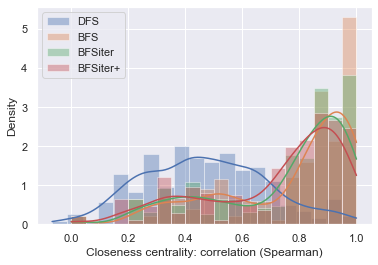
\includegraphics[scale=1.2]{closeness_spearman}
    \caption{Histogram showing the distribution of the Spearman's Rank correlation coefficients of the closeness centrality values computed for the test ligands from the PDBbind-CN data set. It was checked if the closeness centrality of the removed atoms increases during mutation. A 'good' mutation route should show an increase in closeness
centrality because at the beginning the atoms with a high distance
from the other atoms (and hence the CC atoms) and thus a low closeness centrality are removed. When atoms are removed with ascending closeness centrality --- which indicates a 'good' mutation route ---, this leads to a higher positive correlation.  Closeness centrality is computed for the full graph representation, including all CC and dummy atoms. Curves are density estimates of the histograms.}
	\label{fig:closeness_centrality}
\end{figure}


3) Ring-related scores: As stated above, the processing of ring structures
is of crucial importance and pronounced differences between DFS and
BFS occur. Four properties were calculated: The mean asymmetry at
ring opening was measured: After the first atom of a ring structure
is removed, usually two chains emerge. The length difference (i.e.,
the difference in atom number) of these two chains was measured. If
both chains are equally long, the asymmetry is 0. 

The 'asymmetry during ring disassembly'-score does not only evaluate
the first atom removed from a ring, but checks at each mutation step
involving a ring atom if asymmetric chains emerge.

The 'mean number of open rings' indicates how many ring structures
are opened on average, and the 'mean processing time of rings' determines
how many mutation steps it takes to process a ring completely (until
only one atom of the former ring structure is present).

Even using the new algorithms, it is possible 
that a \textquoteleft broken\textquoteright{} ring exists for several mutation steps
 because atoms from other areas of the dummy region (e.g.,
a longer chain) are processed before the ring continues to be processed. However, in contrast to DFS,
it should not happen that a ring near to the CC is opened, but some of its atoms are processed much later, and hence the mean and maximum time should be significantly shorter. 

To compare the mutation algorithms, calculation of the scoring functions for the selection of ligands from the PDBbind-CN data set was performed. 

In general, the computed statistics match the expectations. The range of betweenness centrality scores is much lower for BFS, suggesting that central nodes, i.e., atoms in a ring next to the common core, are processed last, whereas isolated ones, i.e., atoms at the final position of a chain, are processed preferably (fig. \ref{fig:betweenness_centrality}).
Likewise, the correlation between the order of mutation of an atom and its closeness centrality scores is higher for BFS-based approaches because atoms distant from the common core are visited only at the final iterations of the algorithms and so there is a stronger positive correlation between closeness centrality and  mutation order (fig. \ref{fig:closeness_centrality}). For many mutation routes, the correlation of the BFS approaches is almost perfect, i.e., near to one, whereas for DFS it is much lower.
All scoring functions show that the BFS-based algorithms tend to prune the molecule graph at positions more distant from the CC at the beginning of the processing, and rings are processed in a more systematic and 'symmetric' manner (fig. \ref{fig:ring_related}).

In the plots presenting the scoring-functions, all molecule combinations
from the PDBbind-CN data set were used. Thus, the selection of molecule pairs gives rise to CCs and dummy regions with entirely different properties (e.g., number of atoms and presence of cyclic structures) and many  'trivial' structures are over-represented. It could be insightful to use
only a subset (e.g., only molecules with dummy regions involving multiple
ring structures or a minimum number of dummy atoms) or to try even a larger selection from the PDBbind-CN database.




\begin{figure}
	
	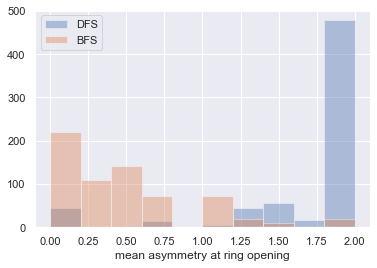
\includegraphics[scale=0.8]{mean_ass_beginn_bfs}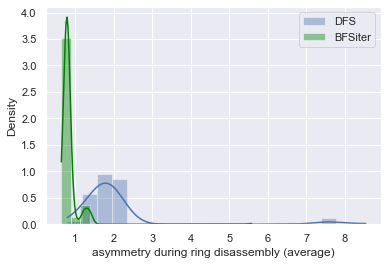
\includegraphics[scale=0.8]{mean_ass_total_onlyiter}
	
	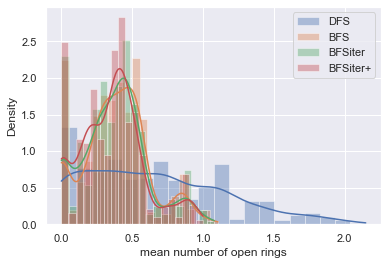
\includegraphics[scale=0.8]{mean_open_rings_all}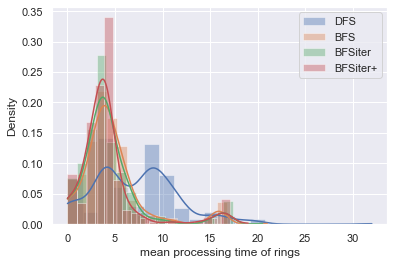
\includegraphics[scale=0.8]{mean_processing_all}
	
	\caption{Ring-related scores for the PDBbind-CN test set. upper row: left: difference in number of atoms in the emerging chains after first removal of a ring atom, a score of 0 means symmetric processing; right: difference in number of atoms in the emerging chains after removal of a ring atom, lower score means more symmetric processing; lower row: left: mean number of open rings in the test molecules after each processing step, lower score means that rings are processed sequentially and not in parallel; right: mean number of mutation steps until a ring is totally processed. Curves are density estimations of the emerging distributions.}
	\label{fig:ring_related}
\end{figure}



\section{Results for selected molecule pairs}

For a selection of small molecules taken from \cite{Loeffler.2018, Wieder.2022}, the relative solvation free energy differences were calculated  using {\trafo} with the old and the new mutation route algorithms. In particular, we studied the three pairs toluene/methane, 2-methylfuran/methane, and 2-methylindole/methane, as well as the
solvation free energy difference between 2-cyclopentyl-indole and 7-cyclopentyl-indole (2-/7-CPI). For the last case, the free energy differences were recomputed only for the new algorithms; however, earlier results using the old algorithm were used for comparison. This is one of the most interesting examples because the old CC generation, which searched for the CC including hydrogens without the improvements reported in 'Processing of hydrogen atoms', generated a smaller CC (fig. \ref{fig:cpi_comparison}). Thus, one would expect that for this example, differences should be especially pronounced.

Although these molecules are rather small and simple, they encompass some of the most interesting features, like rings. For instance, the mutation route for toluene is fundamentally different depending on the algorithm: the old algorithm starts next to the atom of the phenyl group that is connected to the methyl substituent --- which serves as the CC --- and processes the rest of the atoms in a chain-like manner. By contrast, the new one starts at the atom with maximum distance from the substituent and proceeds symmetrically until the CC is reached.
An overview of the molecules and the corresponding mutation routes is shown in figs. \ref{fig:all_paper_molecules} and \ref{fig:cpi_paper_molecule}.
The simulation results are averaged over four runs (except 2-CPI/7-CPI, for which only three runs were performed). 
For all these examples, the standard deviation is smaller using the new route finding algorithm and adapted settings for the generation of the CC (fig. \ref{fig:boxplot_small} and table \ref{tab:results_selection}).

\begin{table}
	\begin{tabular}{|>{\centering}p{5.5cm}|>{\centering}p{3.5cm}|>{\centering}p{3.5cm}|}
		\hline 
		mutation partners & old algorithm (DFS) & new algorithm (BFS) \tabularnewline
		\hline 
		toluene/methane & 2.02 $ \pm $ 0.21 & 2.05 $ \pm $ 0.04 \tabularnewline
		\hline 
		2-methylfuran/methane & 1.47 $ \pm $ 0.24 & 1.60 $ \pm $ 0.16 \tabularnewline
		\hline 	
		2-methyl-1H-indole/methane & 7.85 $ \pm $ 0.23 & 8.20 $ \pm $ 0.13 \tabularnewline
		\hline 	
		
	\end{tabular}\caption{results for a selection of mutation partners }
 \label{tab:results_selection}
\end{table}

\begin{figure}
	
	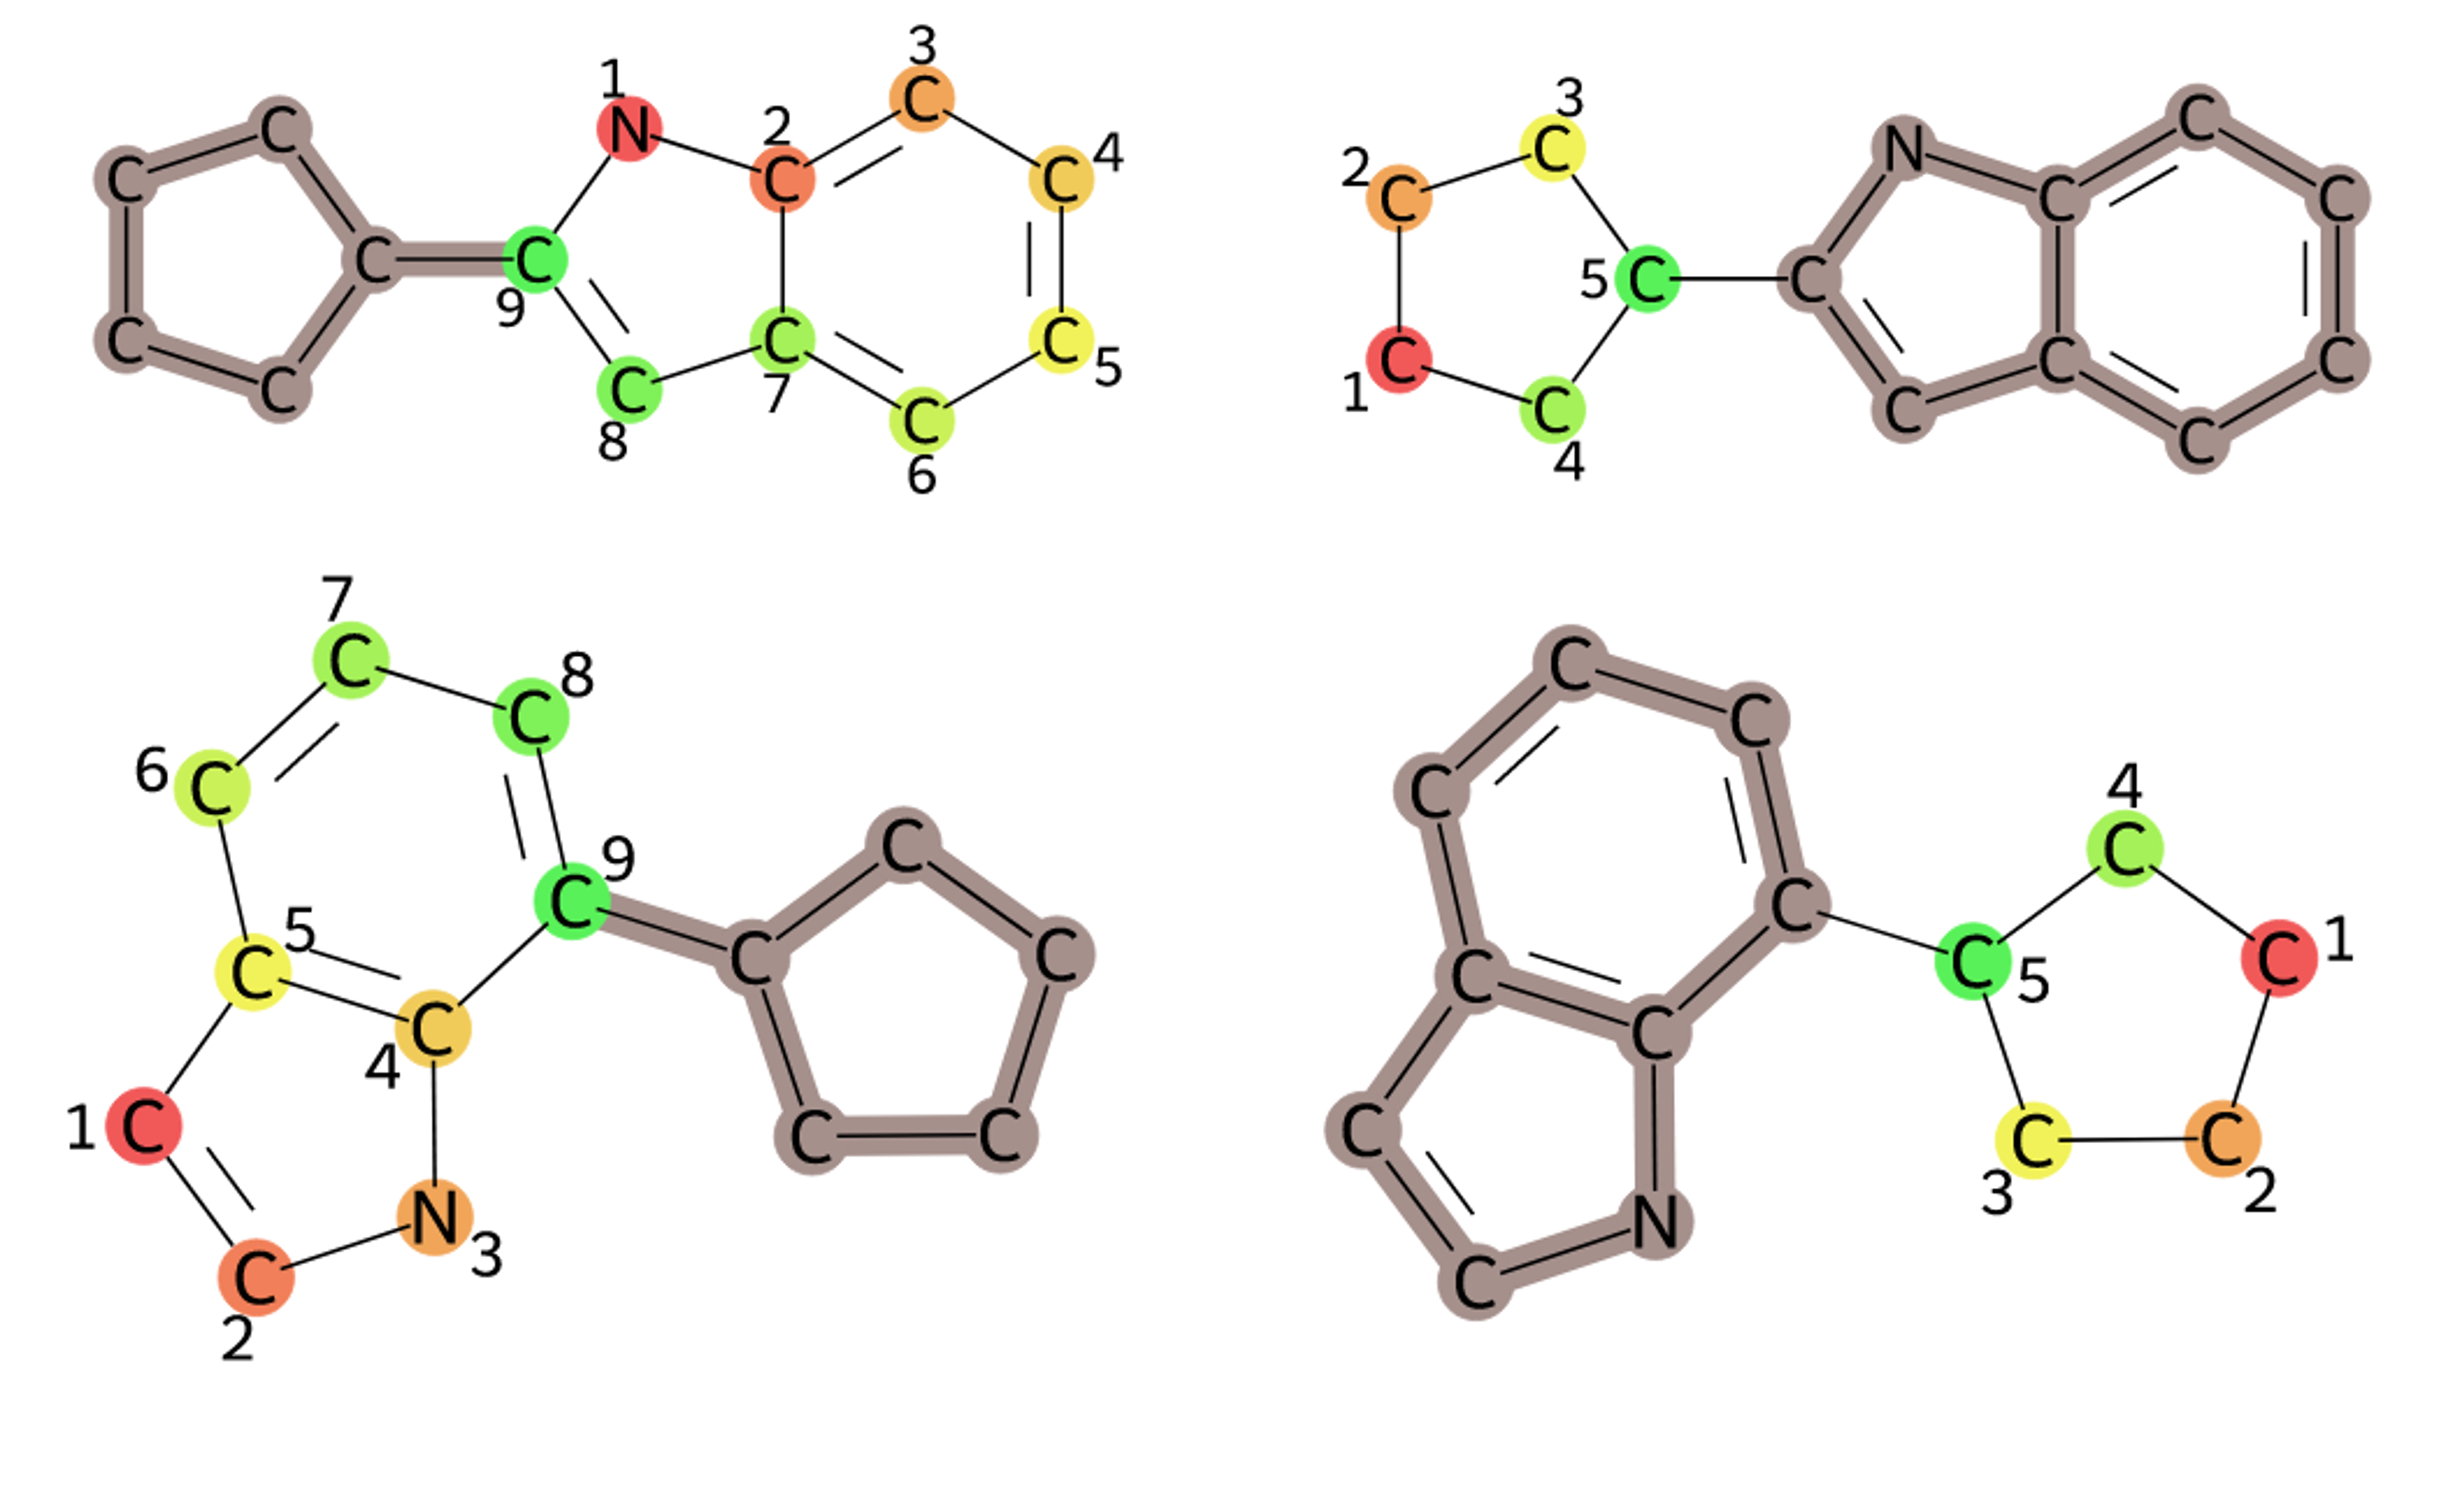
\includegraphics[scale=0.50]{cpi_old_new}
	\caption{mutation routes for 2-cyclopentylindole (upper row)/7-cyclopentylindole (lower row); left: small CC with DFS-algorithm; right: bigger CC with BFS-algorithm; CC in dark; the smaller CC is obtained when hydrogens are not removed before the computation of the maximum common substructure (it should be noted that in this case even further manual post-processing is necessary because one atom of the indole is also attached to the CC)}
	\label{fig:cpi_comparison}
\end{figure}



\begin{figure}
	
	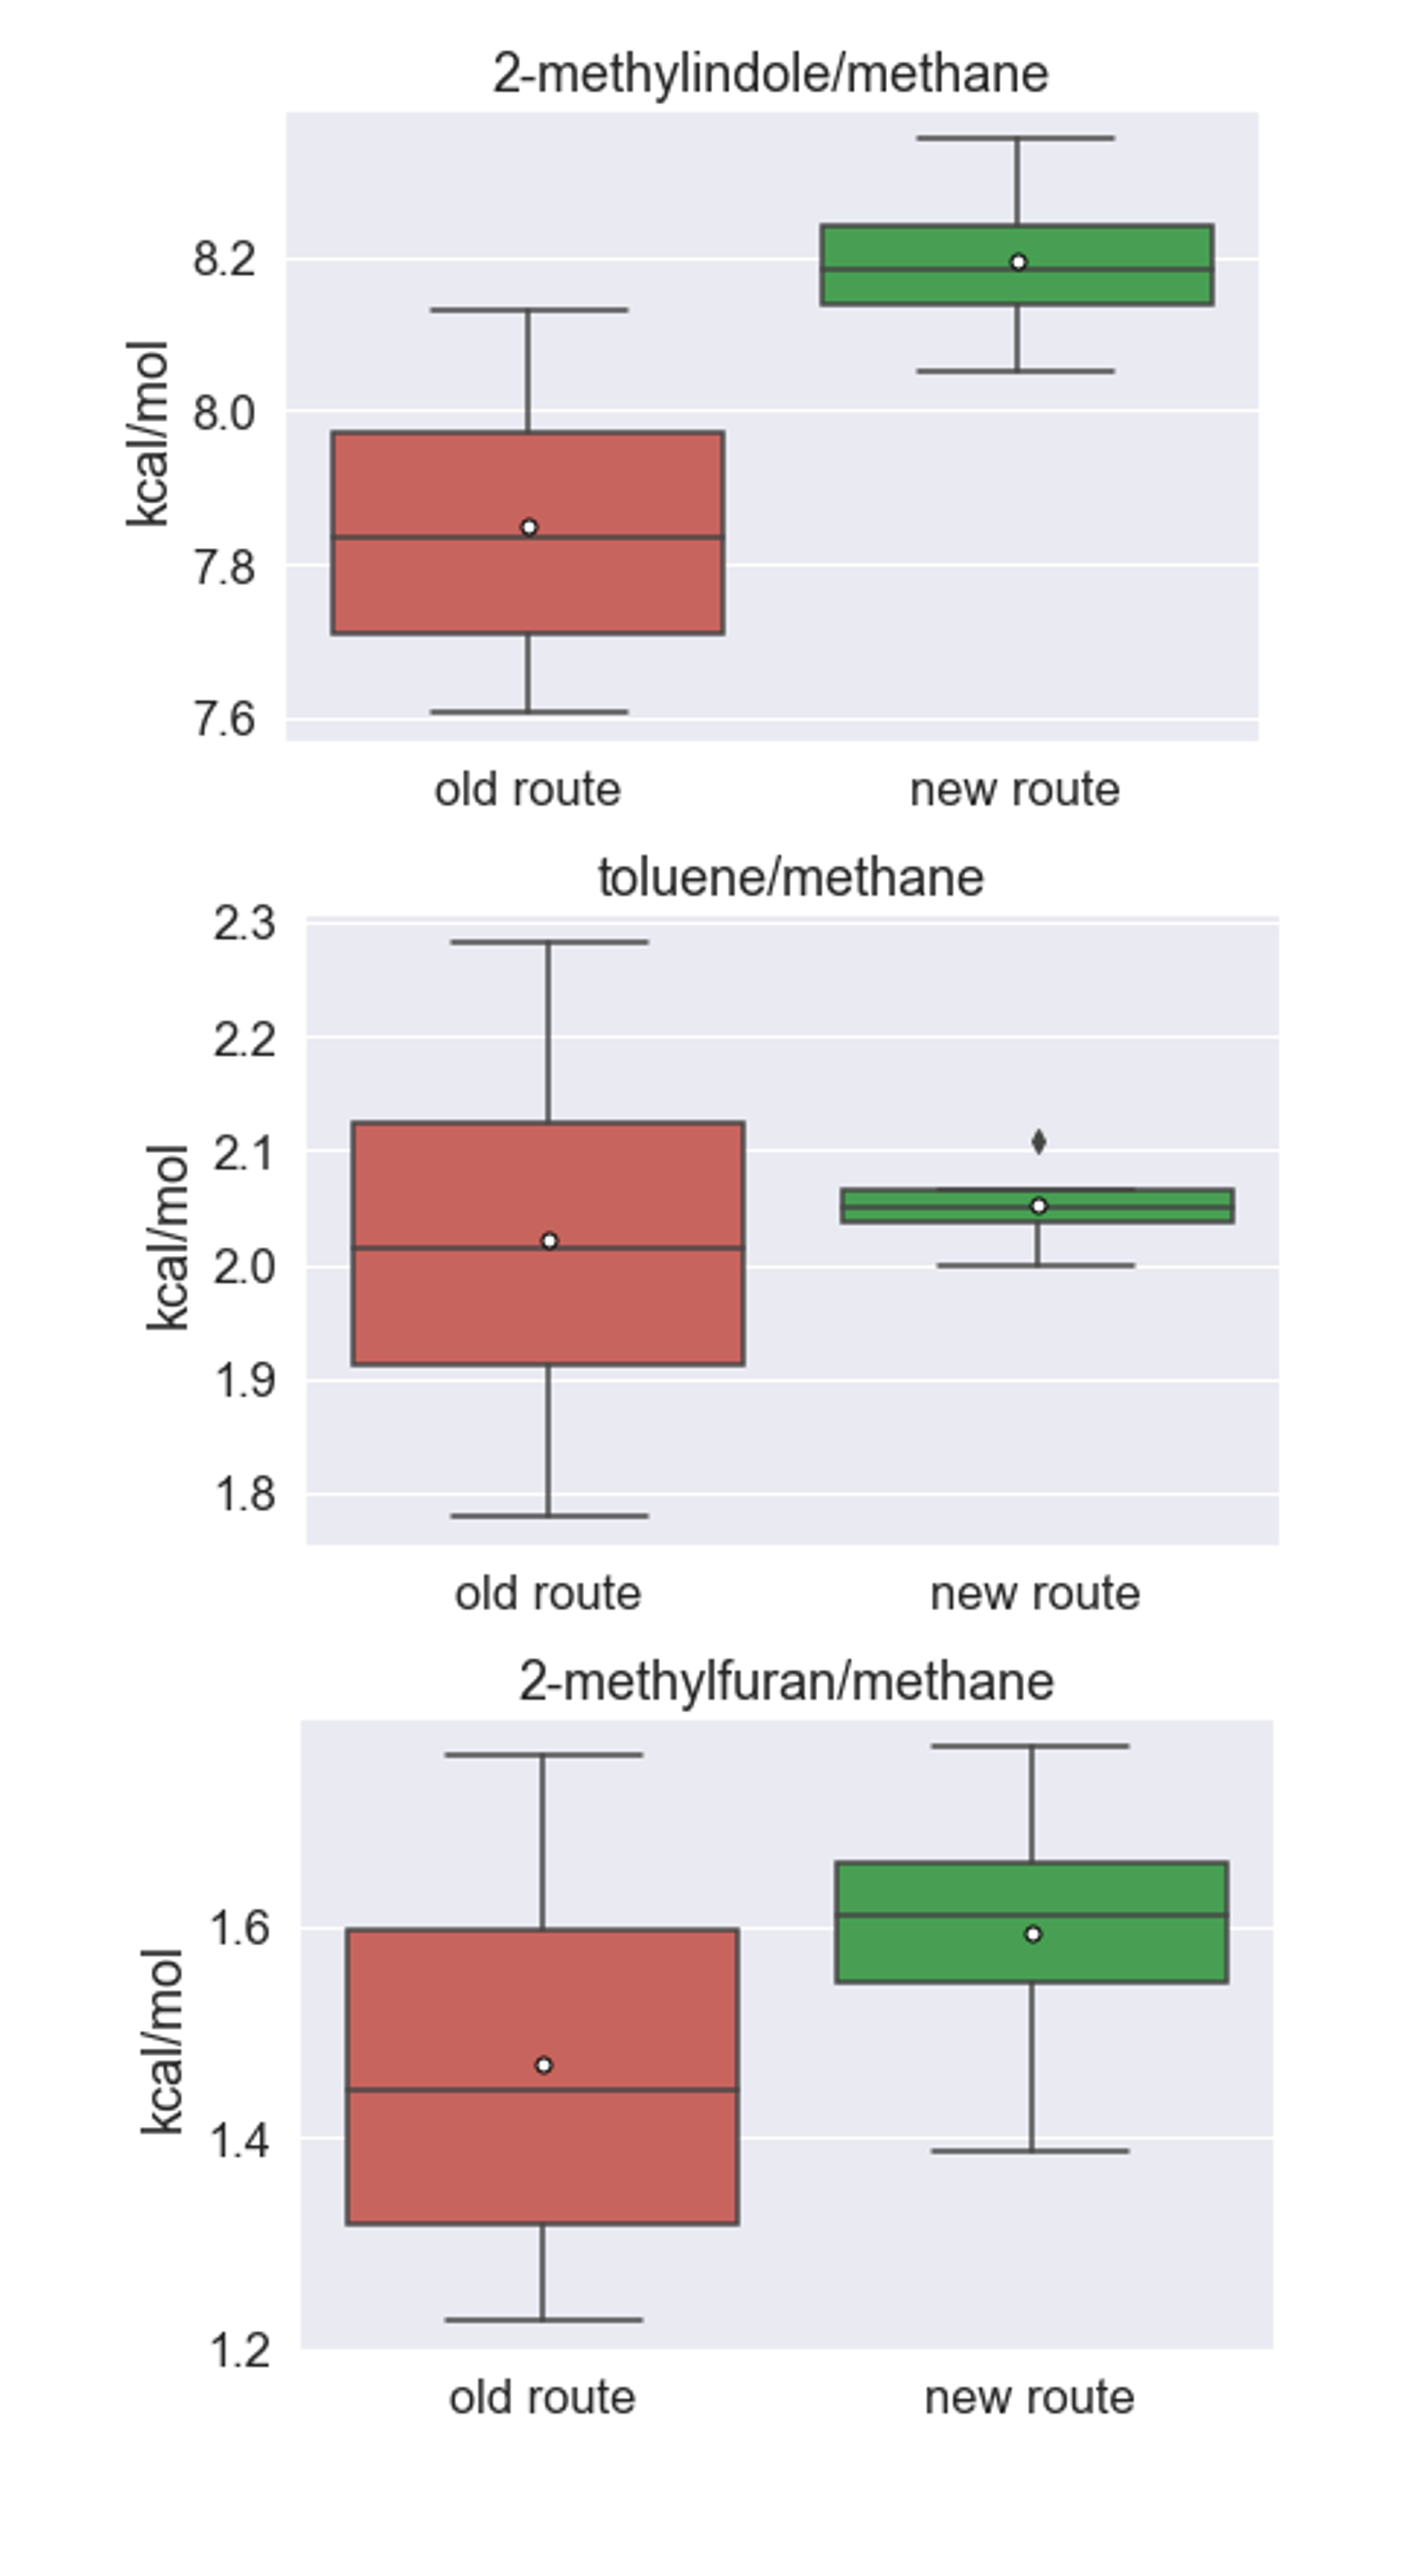
\includegraphics[scale=0.65]{results_3pairs1}
	\caption{comparison of results for mutating 2-methylindole, toluene and 2-methylfuran to methane.}
	\label{fig:boxplot_small}
\end{figure}


For the 2-/7-CPI-transformation, a relative free energy difference of $-1.55 \pm  0.10$ kcal/mol is computed using the CC and the route proposed by the new algorithms. In \cite{Fleck.2021}, for this transformation, $-1.43  \pm $ 0.30 kcal/mol was determined with the smaller cyclopentane-X CC. It can be assumed that the differences between the old and new mutation route are even more pronounced because in \cite{Fleck.2021} the calculations were repeated five times and averaged, in contrast to only three replicates for the run with the new mutation route. 
Of course, a direct comparison with the same number of replicates would be advantageous to quantify the improvement, but in any case, the change in standard deviation is remarkable.
Calculation of the absolute free energy differences of both molecules yield $-1.58  \pm  0.30$~kcal/mol. This indicates that the new route not only provides a smaller error, but also leads to a more accurate result.

However, probably the greatest advantage is that the mutation route for the new, bigger CC needs fewer states (only five in contrast to nine heavy atoms have to be mutated). 




\begin{figure}[h]
	\centering
	\subfigure[toluene/vacuum old]{%
		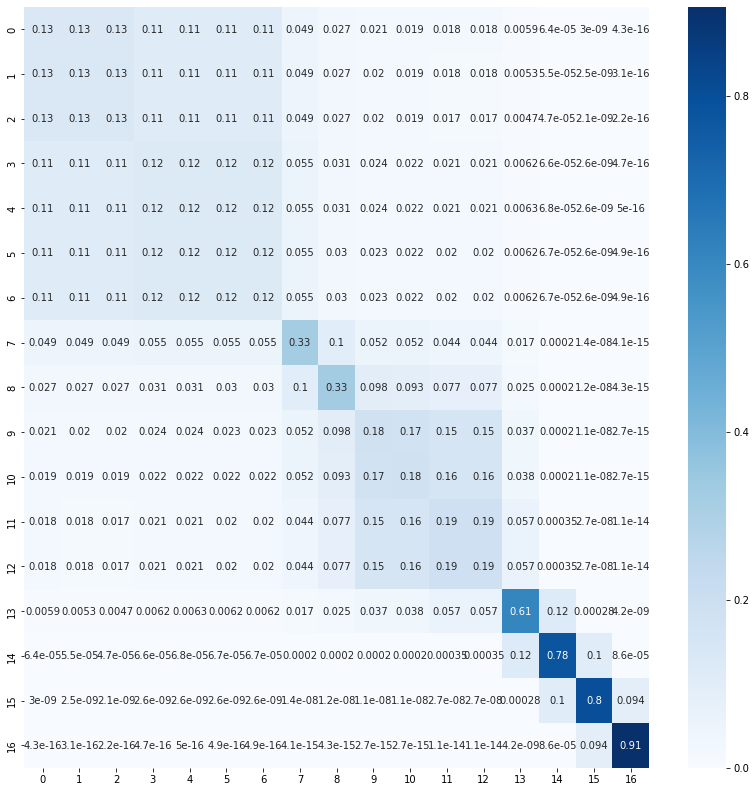
\includegraphics[width=0.5\textwidth]{overlap_vacuum_toluene_old_v2}%
		\label{fig:v_toluene_old}%
	}\hfil
	\subfigure[toluene/vacuum new]{%
		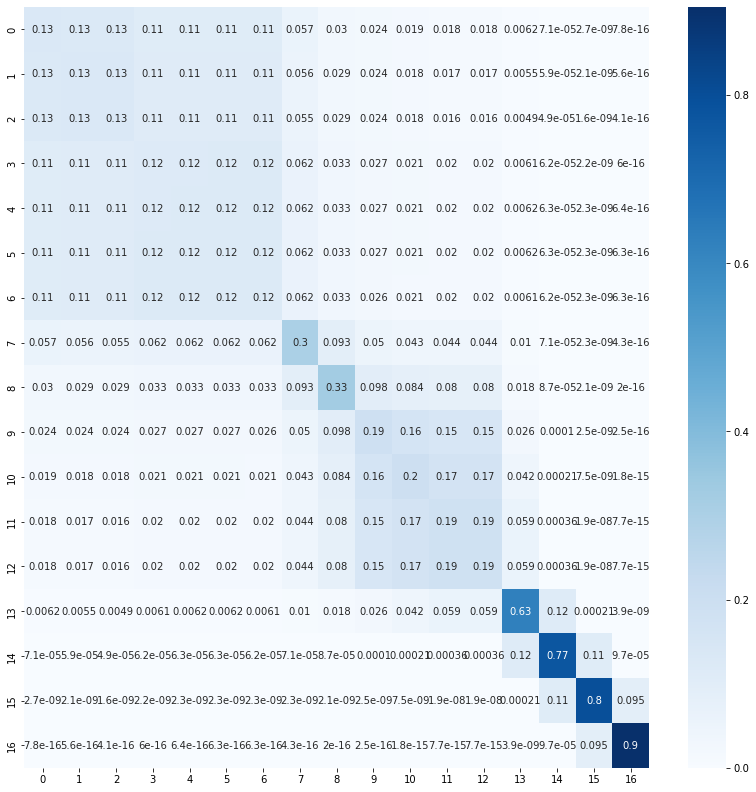
\includegraphics[width=0.5\textwidth]{overlap_vacuum_toluene_new_v2}%
		\label{fig:v_toluene_new}%
	}
	
	\subfigure[toluene/waterbox old]{%
		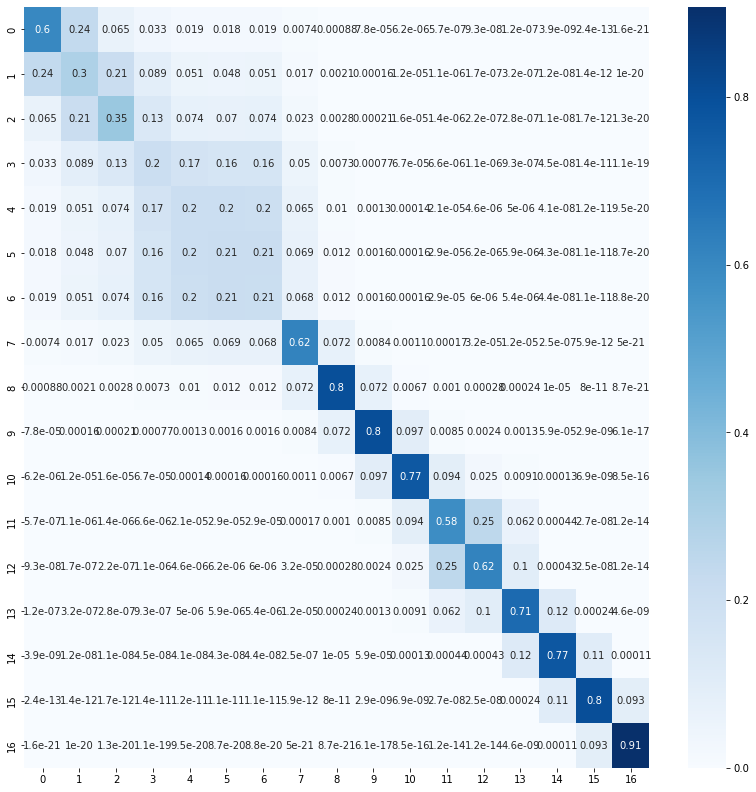
\includegraphics[width=0.5\textwidth]{overlap_waterbox_toluene_old_v2}%
		\label{fig:w_toluene_old}%
	}\hfil
	\subfigure[toluene/waterbox new]{%
		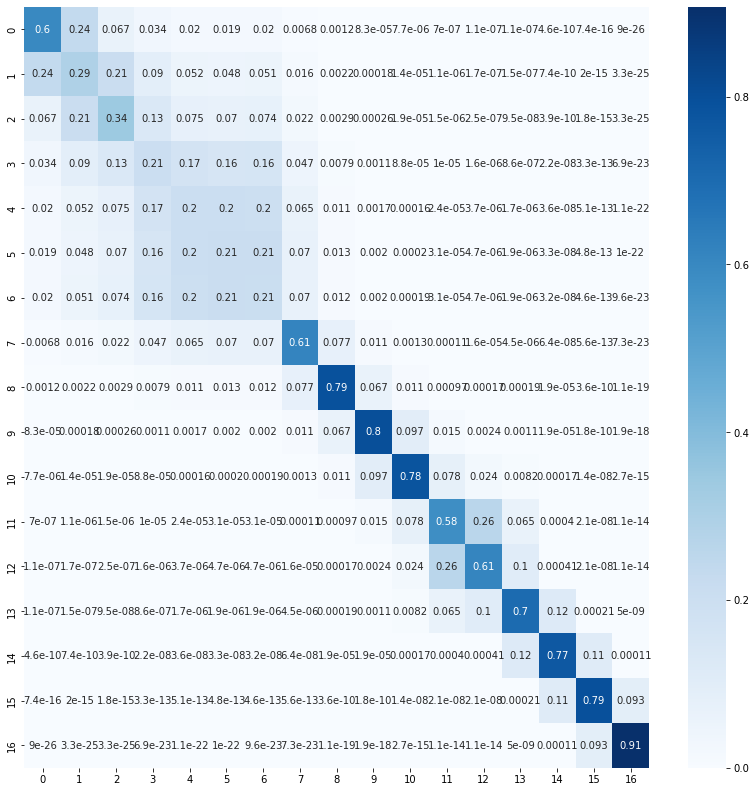
\includegraphics[width=0.5\textwidth]{overlap_waterbox_toluene_new_v2}%
		\label{fig:w_toluene_new}%
	}
	
	\caption{Overlap plots for toluene $\mathrm{\rightarrow}$ methane: upper row: vacuum, lower row: water box; left: old mutation algorithm, right: new mutation algorithm}
	\label{fig:toluene_overlaps}
\end{figure}


\begin{figure}[h]
	\centering
	\subfigure[toluene/vacuum old]{%
		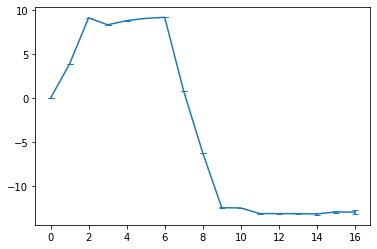
\includegraphics[width=0.55\textwidth]{states_toluene_vacuum_old_v2.png}%
		\label{fig:v_toluene_old_state}%
	}\hfil
	\subfigure[toluene/vacuum new]{%
		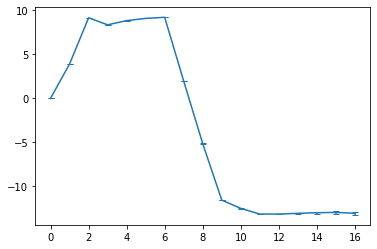
\includegraphics[width=0.55\textwidth]{states_toluene_vacuum_new_v2.png}%
		\label{fig:v_toluene_new_state}%
	}
	
	\subfigure[toluene/waterbox old]{%
		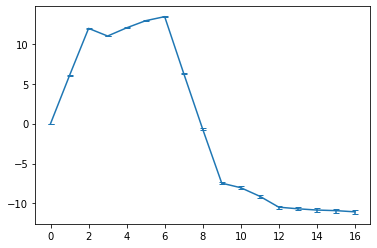
\includegraphics[width=0.55\textwidth]{states_toluene_water_old_v2.png}%
		\label{fig:w_toluene_old_state}%
	}\hfil
	\subfigure[toluene/waterbox new]{%
		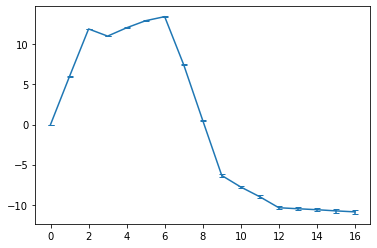
\includegraphics[width=0.55\textwidth]{states_toluene_water_new_v2.png}%
		\label{fig:w_toluene_new_state}%
	}
	
	\caption{free energy differences per state for toluene $\mathrm{\rightarrow}$ methane}
	\label{fig:toluene_states}
\end{figure}

\begin{figure}[h]
	\centering
	\subfigure[toluene/vacuum old]{%
		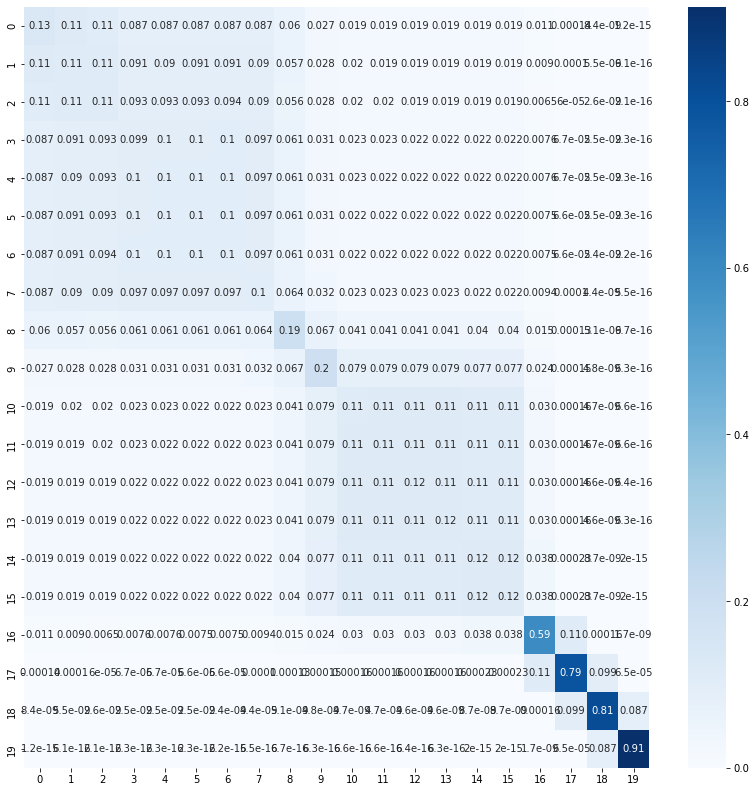
\includegraphics[width=0.5\textwidth]{overlap_vacuum_methylindole_old_v2}%
		\label{fig:v_methylindole_old}%
	}\hfil
	\subfigure[toluene/vacuum new]{%
		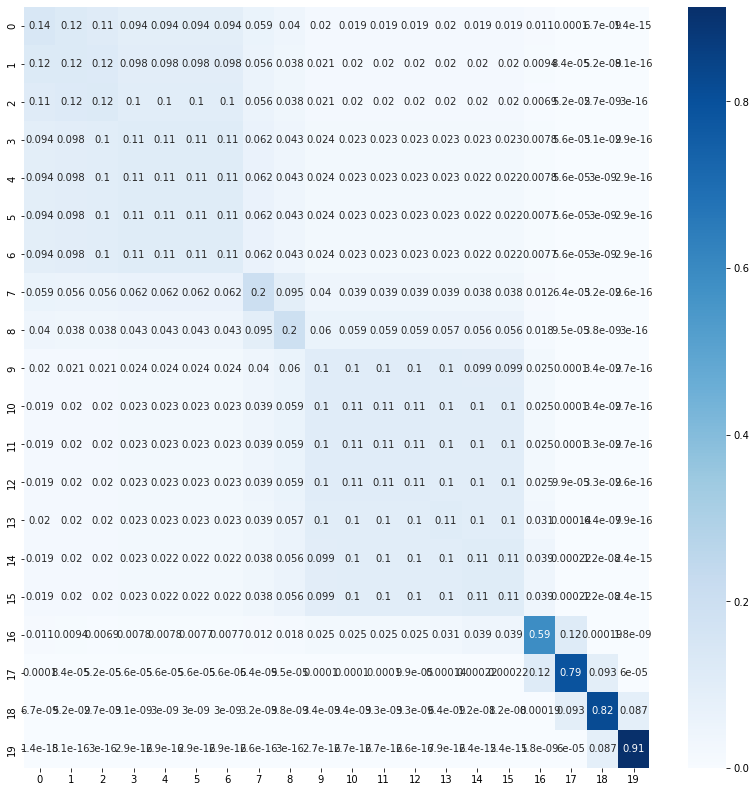
\includegraphics[width=0.5\textwidth]{overlap_vacuum_methylindole_new_v2}%
		\label{fig:v_methylindole_new}%
	}
	
	\subfigure[toluene/waterbox old]{%
		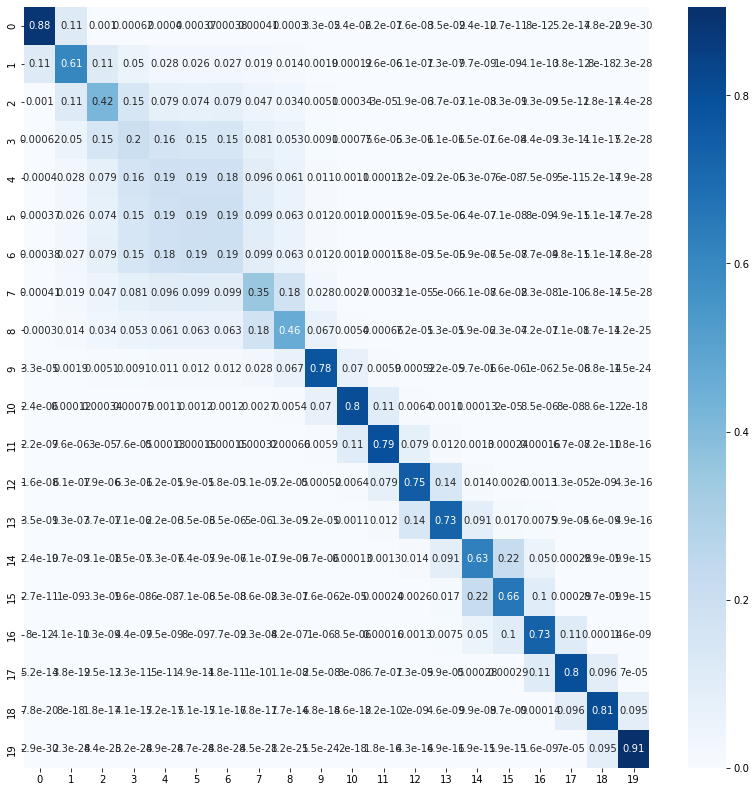
\includegraphics[width=0.5\textwidth]{overlap_waterbox_methylindole_old_v2}%
		\label{fig:w_methylindole_old}%
	}\hfil
	\subfigure[toluene/waterbox new]{%
		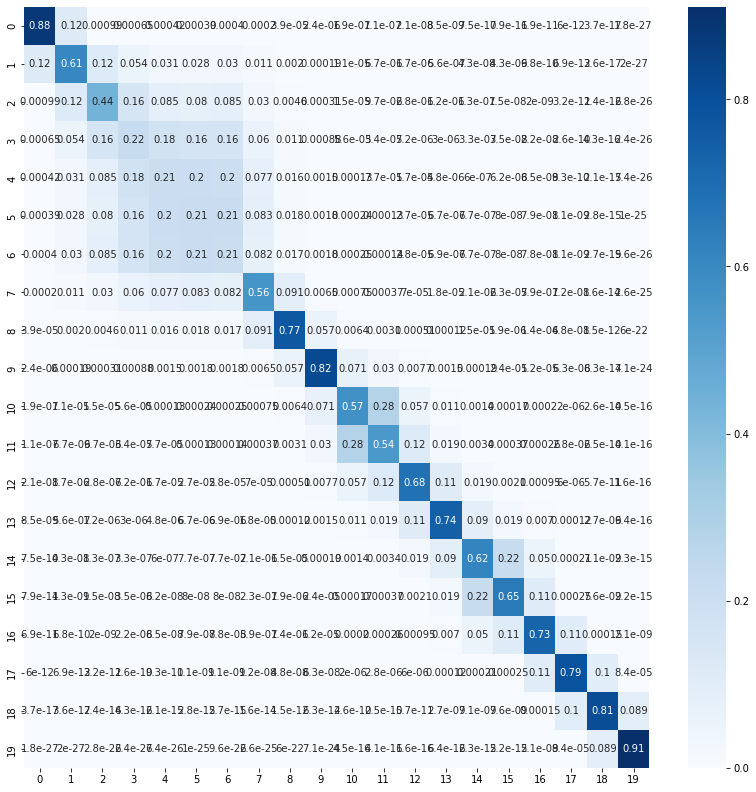
\includegraphics[width=0.5\textwidth]{overlap_waterbox_methylindole_new_v2}%
		\label{fig:w_methylindole_new}%
	}
	
	\caption{Overlap plots for 2-methyl-1H-indole $\mathrm{\rightarrow}$ methane: upper row: vacuum, lower row: water box; left: old mutation algorithm, right: new mutation algorithm}
	\label{fig:methylindole_overlaps}
\end{figure}


\begin{figure}[!htb]
	
	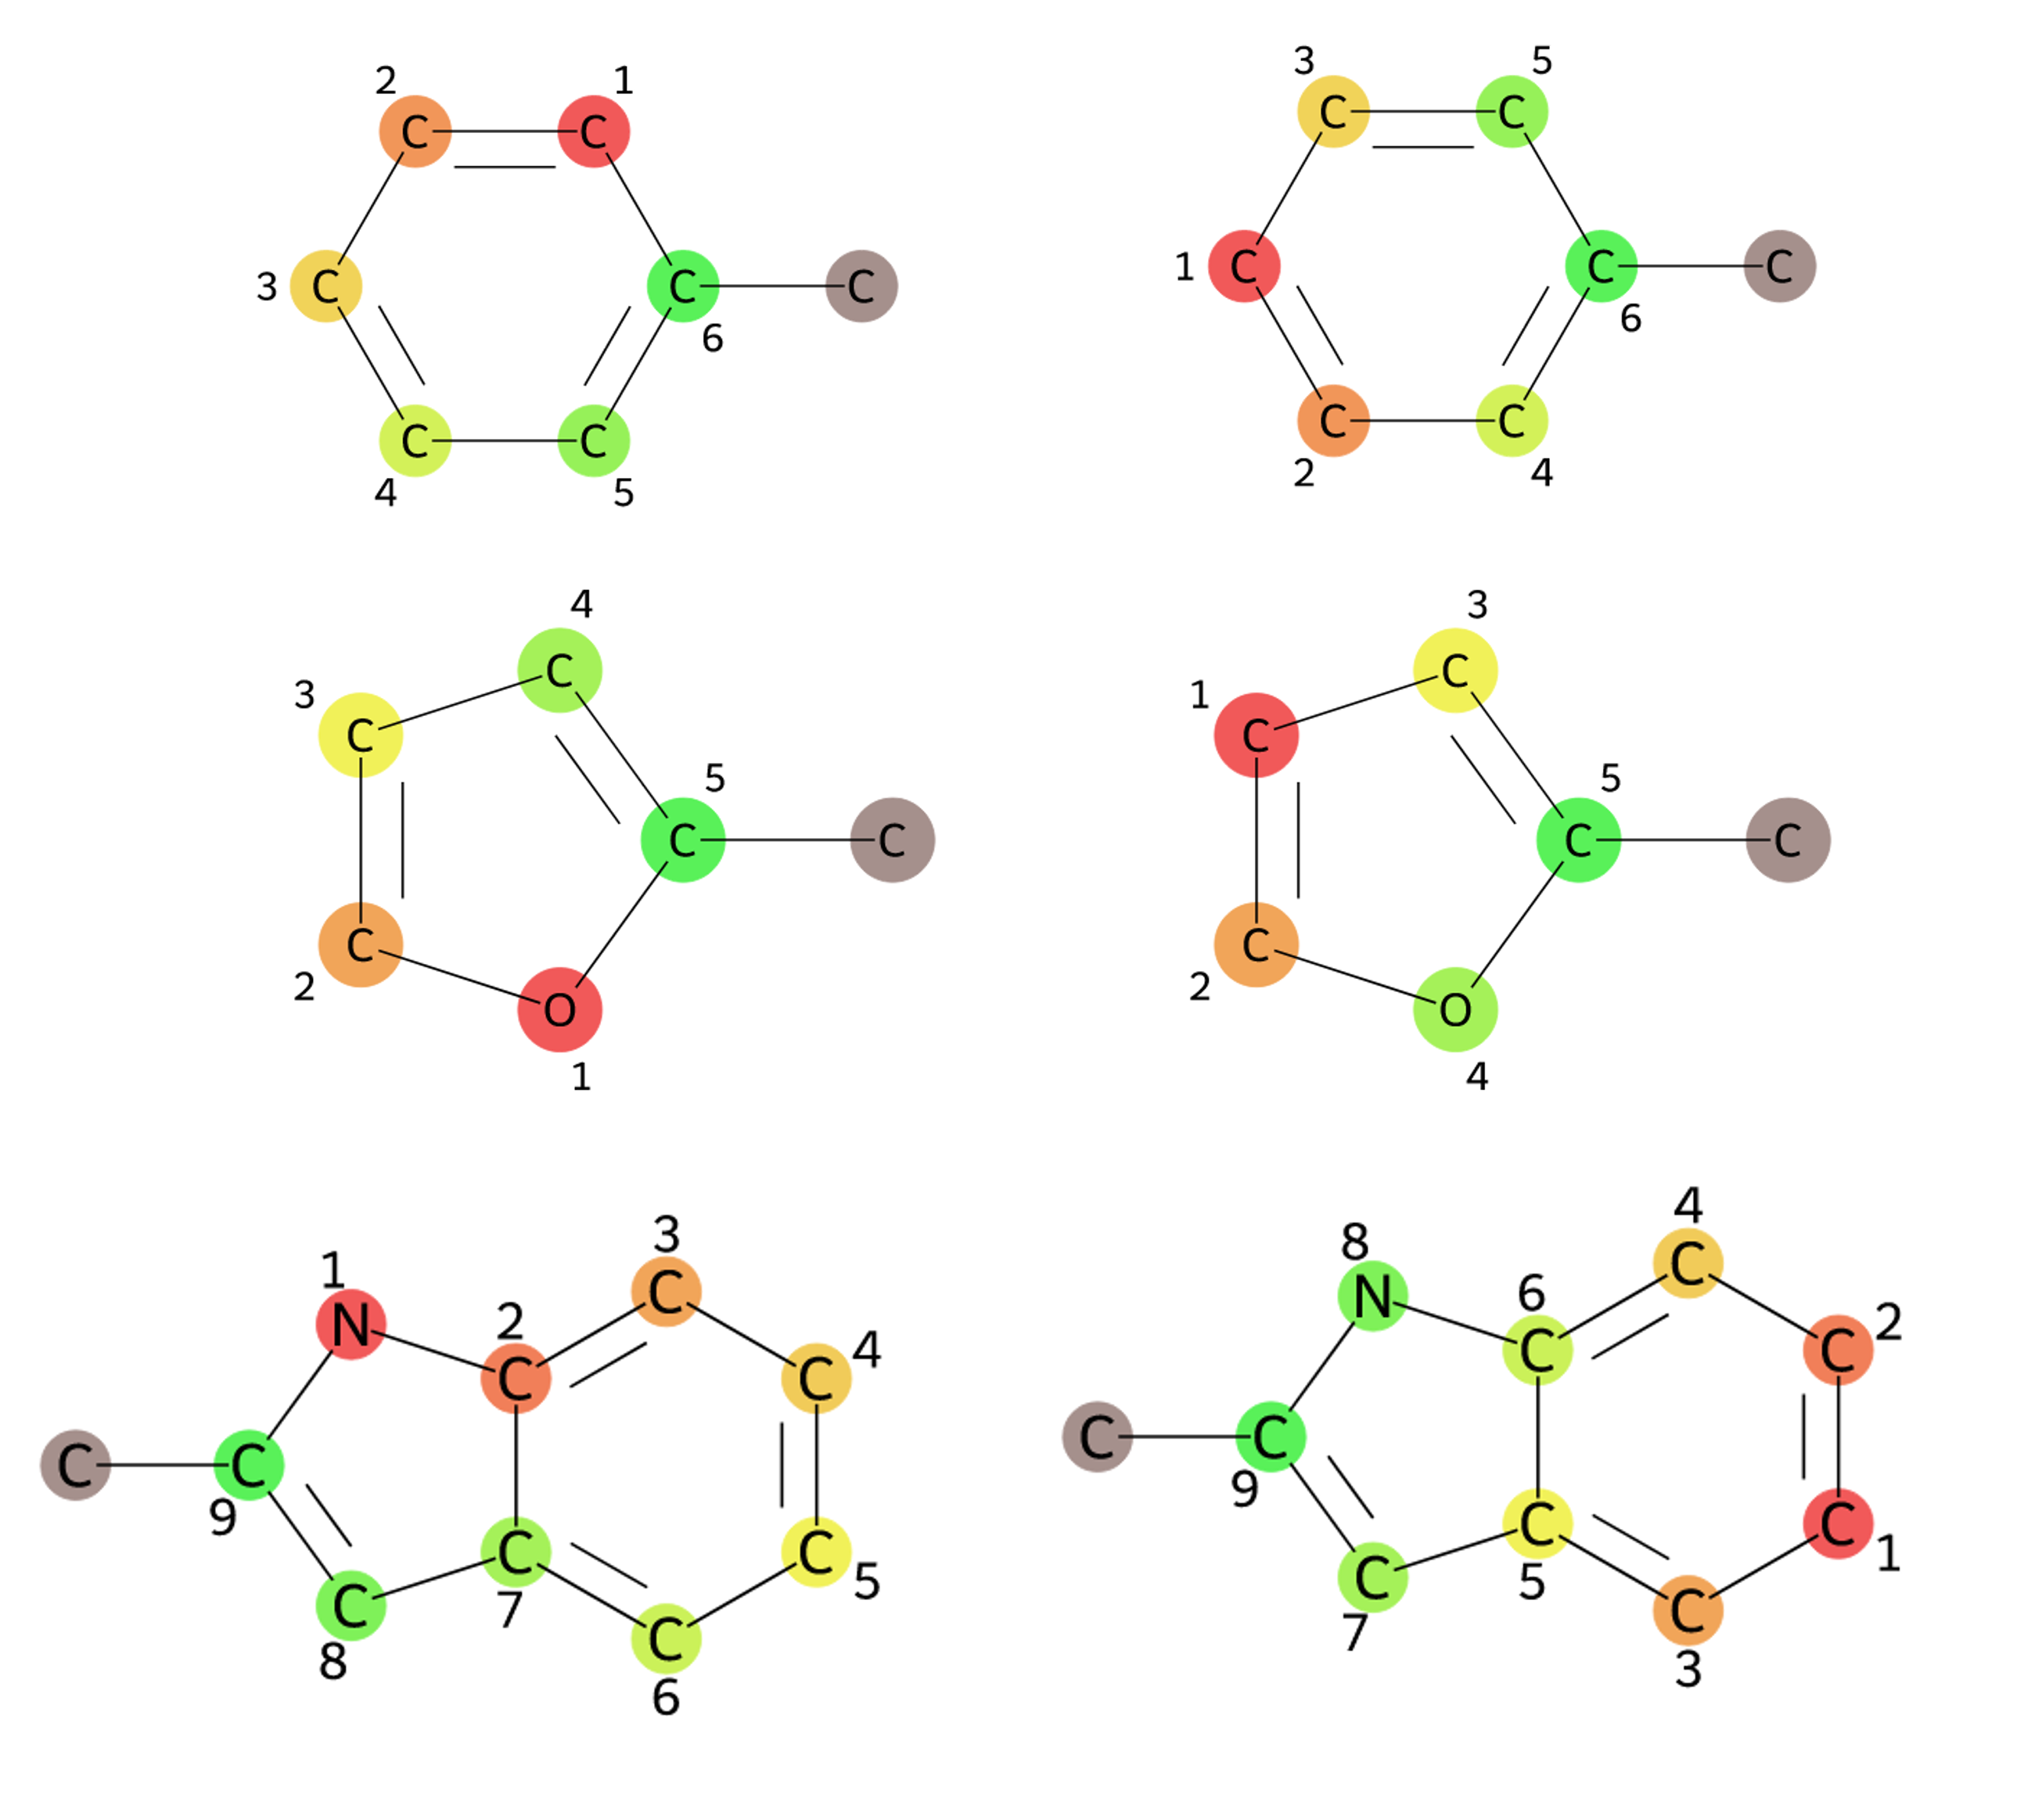
\includegraphics[scale=0.75]{paper_routes1a}\caption{left: DFS-algorithm; right: BFS-algorithm; CC in dark; from top to bottom row: mutation routes for toluene/methane, 2-methylfuran/methane, 2-methylindole/methane}
	\label{fig:all_paper_molecules}
\end{figure}


\begin{figure}[!htb]
	
	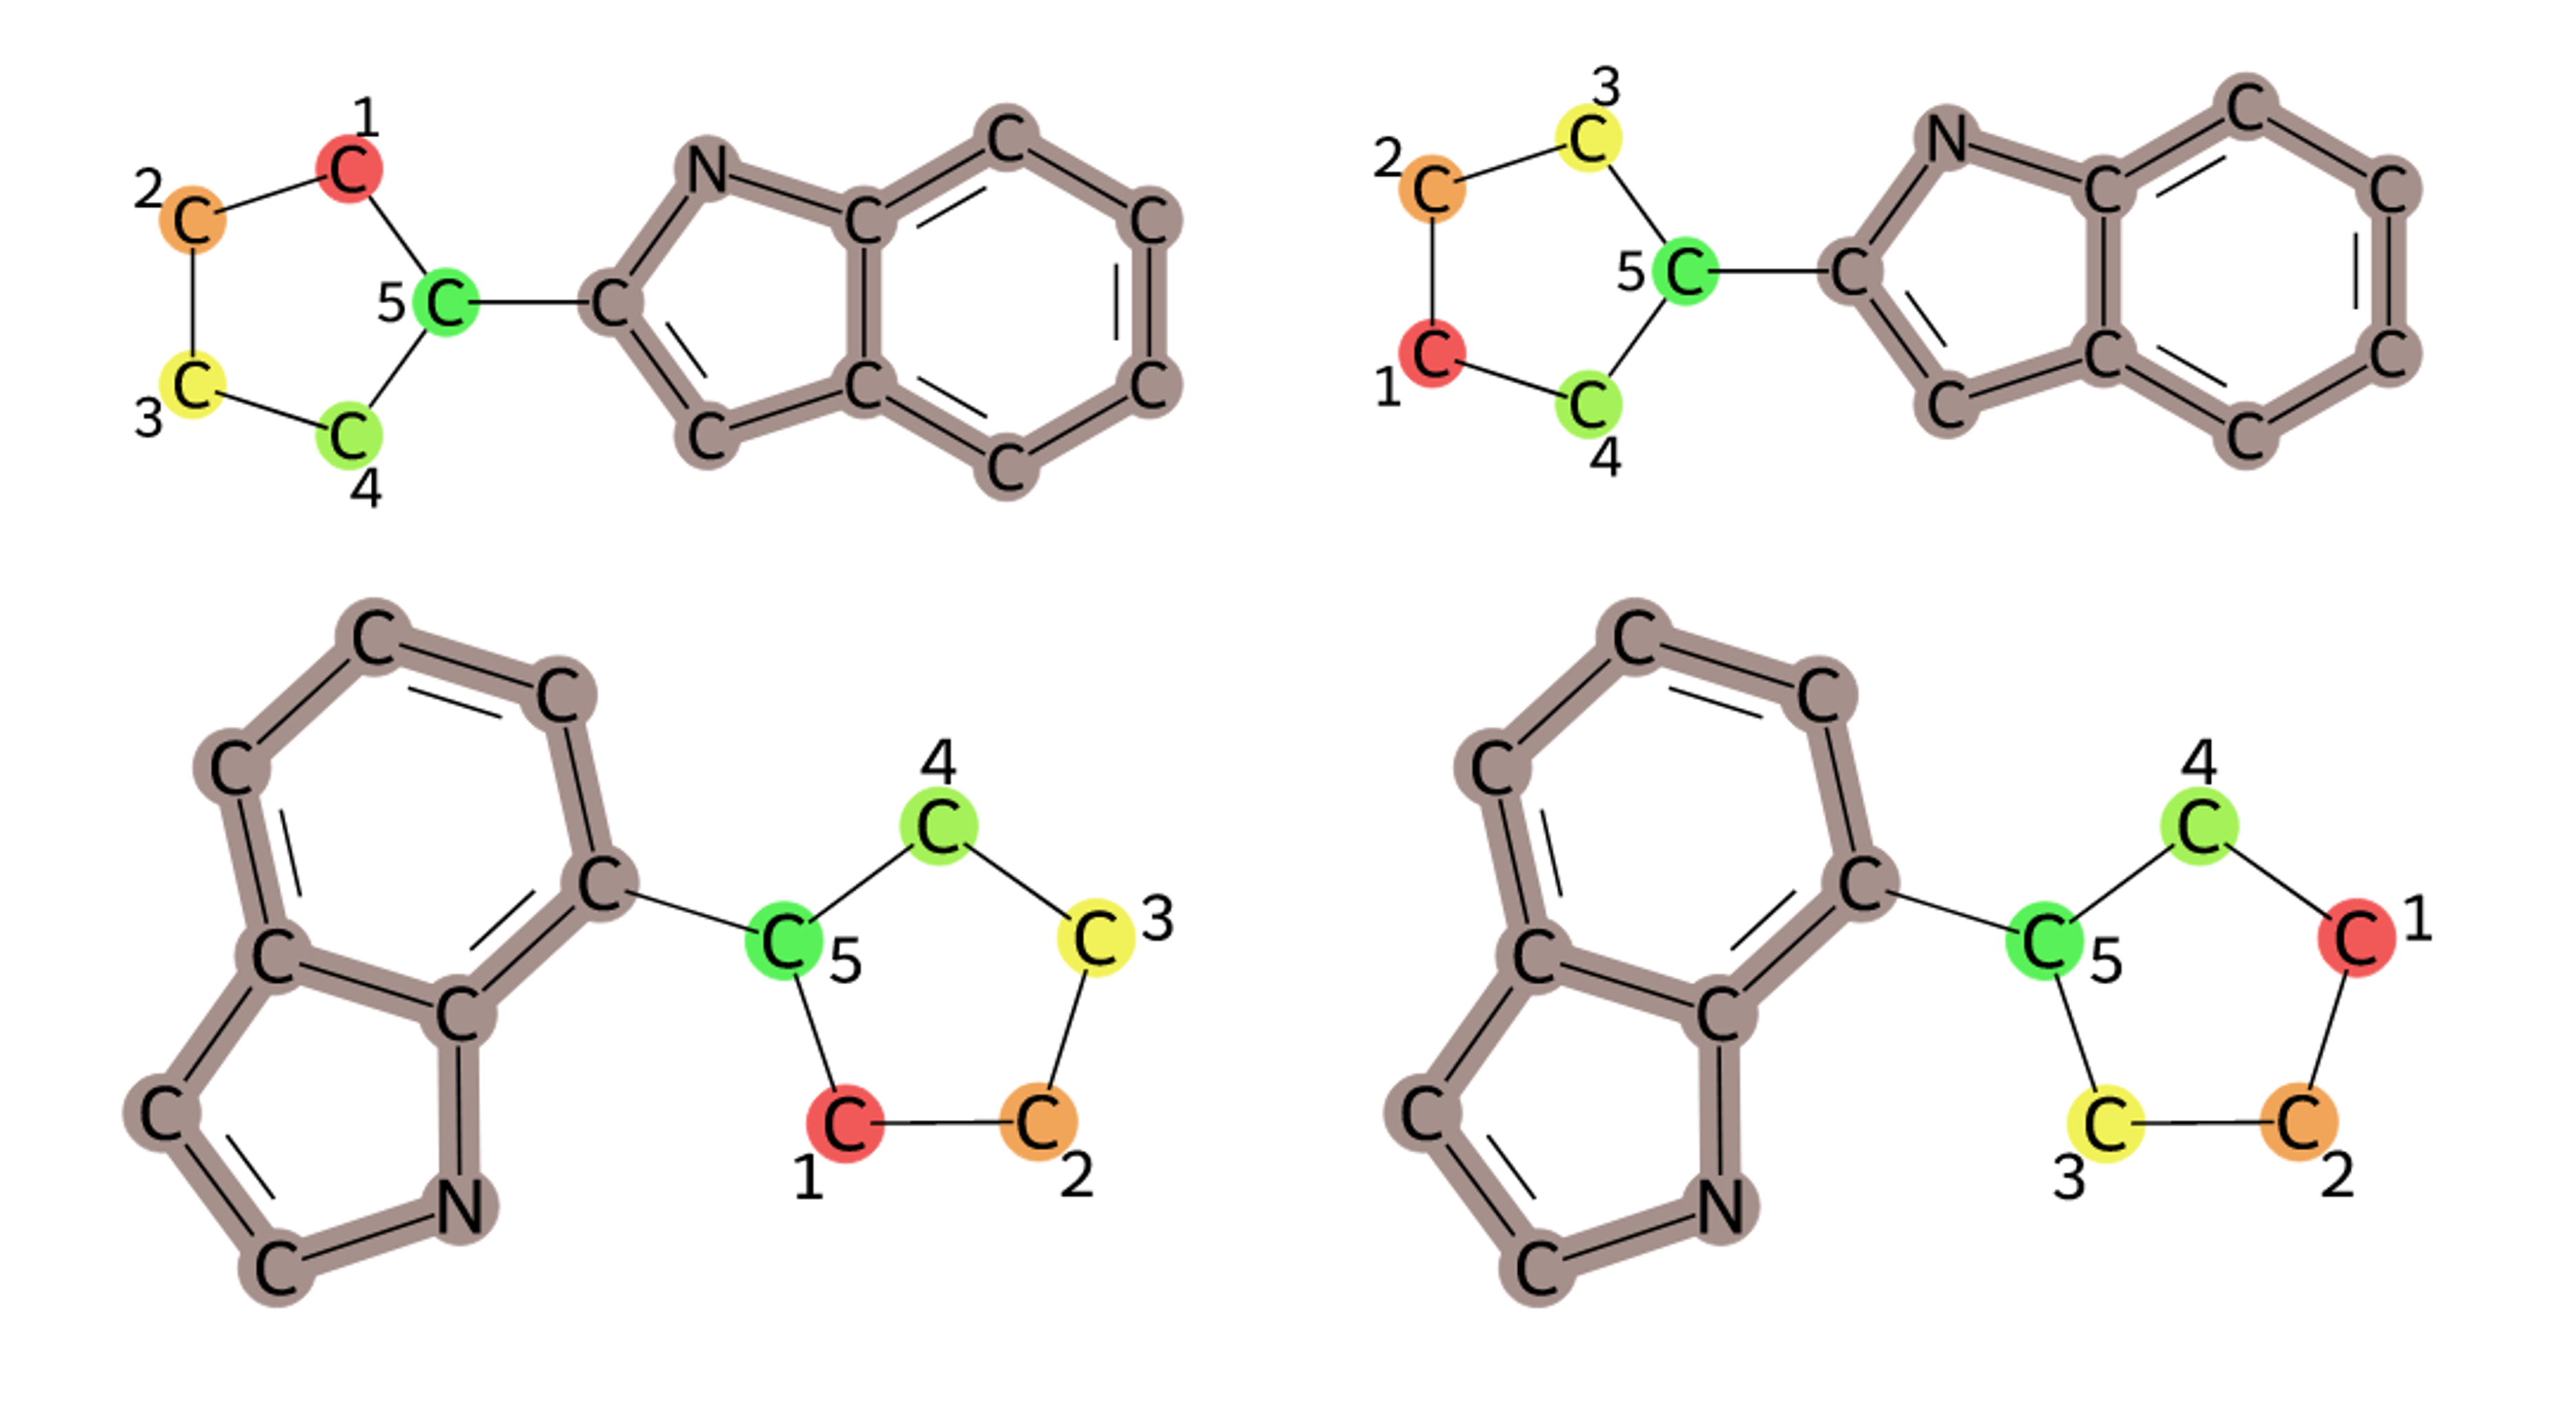
\includegraphics[scale=0.55]{paper_routes1b}\caption{left: DFS-algorithm; right: BFS-algorithm; CC in dark; mutation routes for 2-cyclopentylindole/7-cyclopentylindole}
	\label{fig:cpi_paper_molecule}
\end{figure}


An additional means for detecting differences between the outcome of the mutation algorithms is to compare runs of different sampling length. 
The results of the MD runs set up with {\trafo} can be evaluated using the functions of the MBAR class of \texttt{pymbar} \cite{Shirts.2008}. Python scripts were written to evaluate the computed free energy differences for different simulation lengths. There are two crucial parameters: the reduced potential energy of an uncorrelated configuration $n$ at a specific state $k$ (\texttt{u\_kn}) and the number of uncorrelated snapshots $n$ (\texttt{N\_k}). By removing the same number of configurations at each state k and adjusting (\texttt{N\_k}) accordingly, shorter simulations were generated artificially.
In \ref{fig:toluene_short}, \ref{fig:methylfuran_short} and \ref{fig:methylindole_short}, a comparison between old and new route for molecule pairs consisting of toluene, 2-methylfuran, 2-methyl-1H-indole and methane is presented. The mean of the calculated free energy differences as well as the standard deviation is shown. In \ref{fig:cpi_short}, free energy differences for the 2-CPI-mutations at the two conditions (water box and vacuum) are visualized. 
As expected, for longer simulation lengths the standard deviation decreases, whereas very short simulation lengths (i.e., a very low number of configuration snapshots as input for the MBAR computations using \texttt{pymbar}) lead to unreliable results. However, looking at the evolution of the free energy difference mean value and standard deviation, it is difficult to confirm the superiority of one of the mutation routes for these three transformations or to indicate a sufficient minimum simulation length.
Furthermore, the \texttt{pymbar}-package \cite{Shirts.2008} allows the computation of overlap plots. Figs. \ref{fig:toluene_overlaps}, \ref{fig:toluene_states}, and \ref{fig:methylindole_overlaps} show overlap plots and the change of free energy difference of one run between the states for toluene $\mathrm{\rightarrow}$ methane and overlap plots for 2-methyl-1H-indole. In the case of 2-methyl-1H-indole (the mutation involves processing of a double ring),  significant differences for the water box between the old and new algorithm are discernible.



\begin{figure}[!htb]
	
	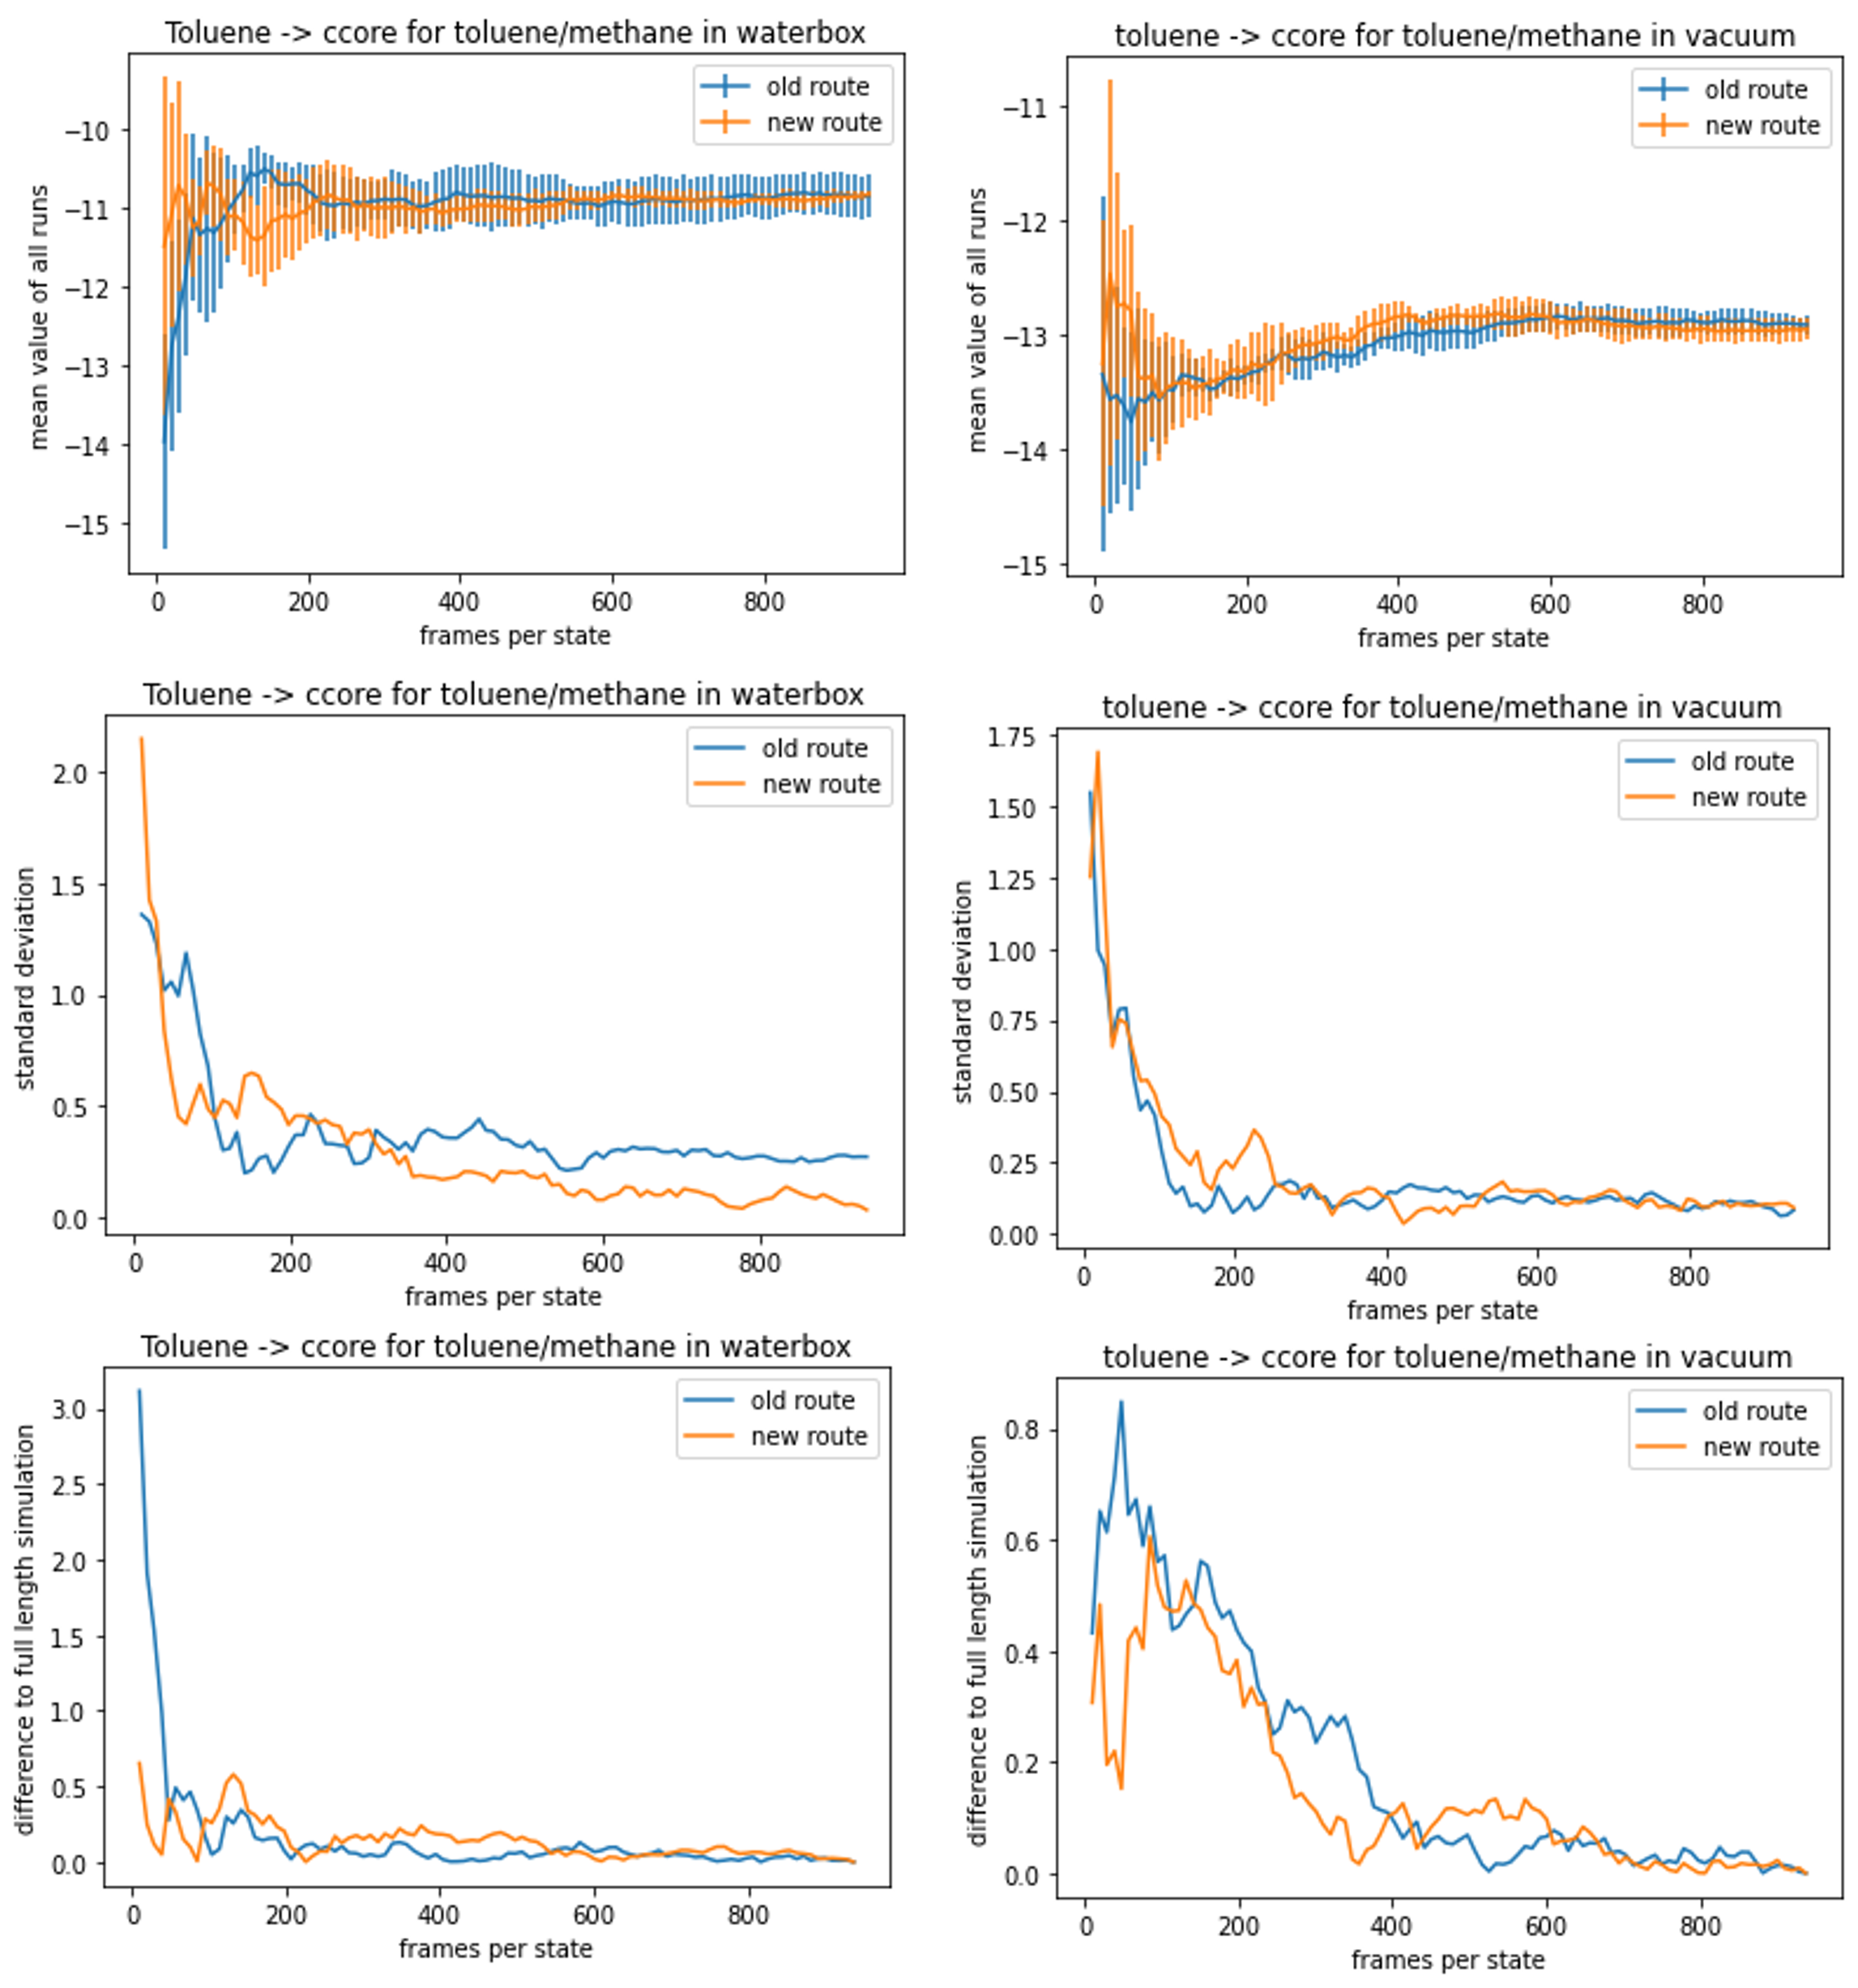
\includegraphics[scale=0.9]{toluene_short}\caption{toluene $\mathrm{\rightarrow}$ methane; left: water box; right: vacuum; mutation routes for toluene/methane; first row: mean value, bars indicate standard deviation; middle row: standard deviation; third row: difference to full-length simulation (i.e., the last value is zero)}
		\label{fig:toluene_short}
\end{figure}

\begin{figure}[!htb]
	
	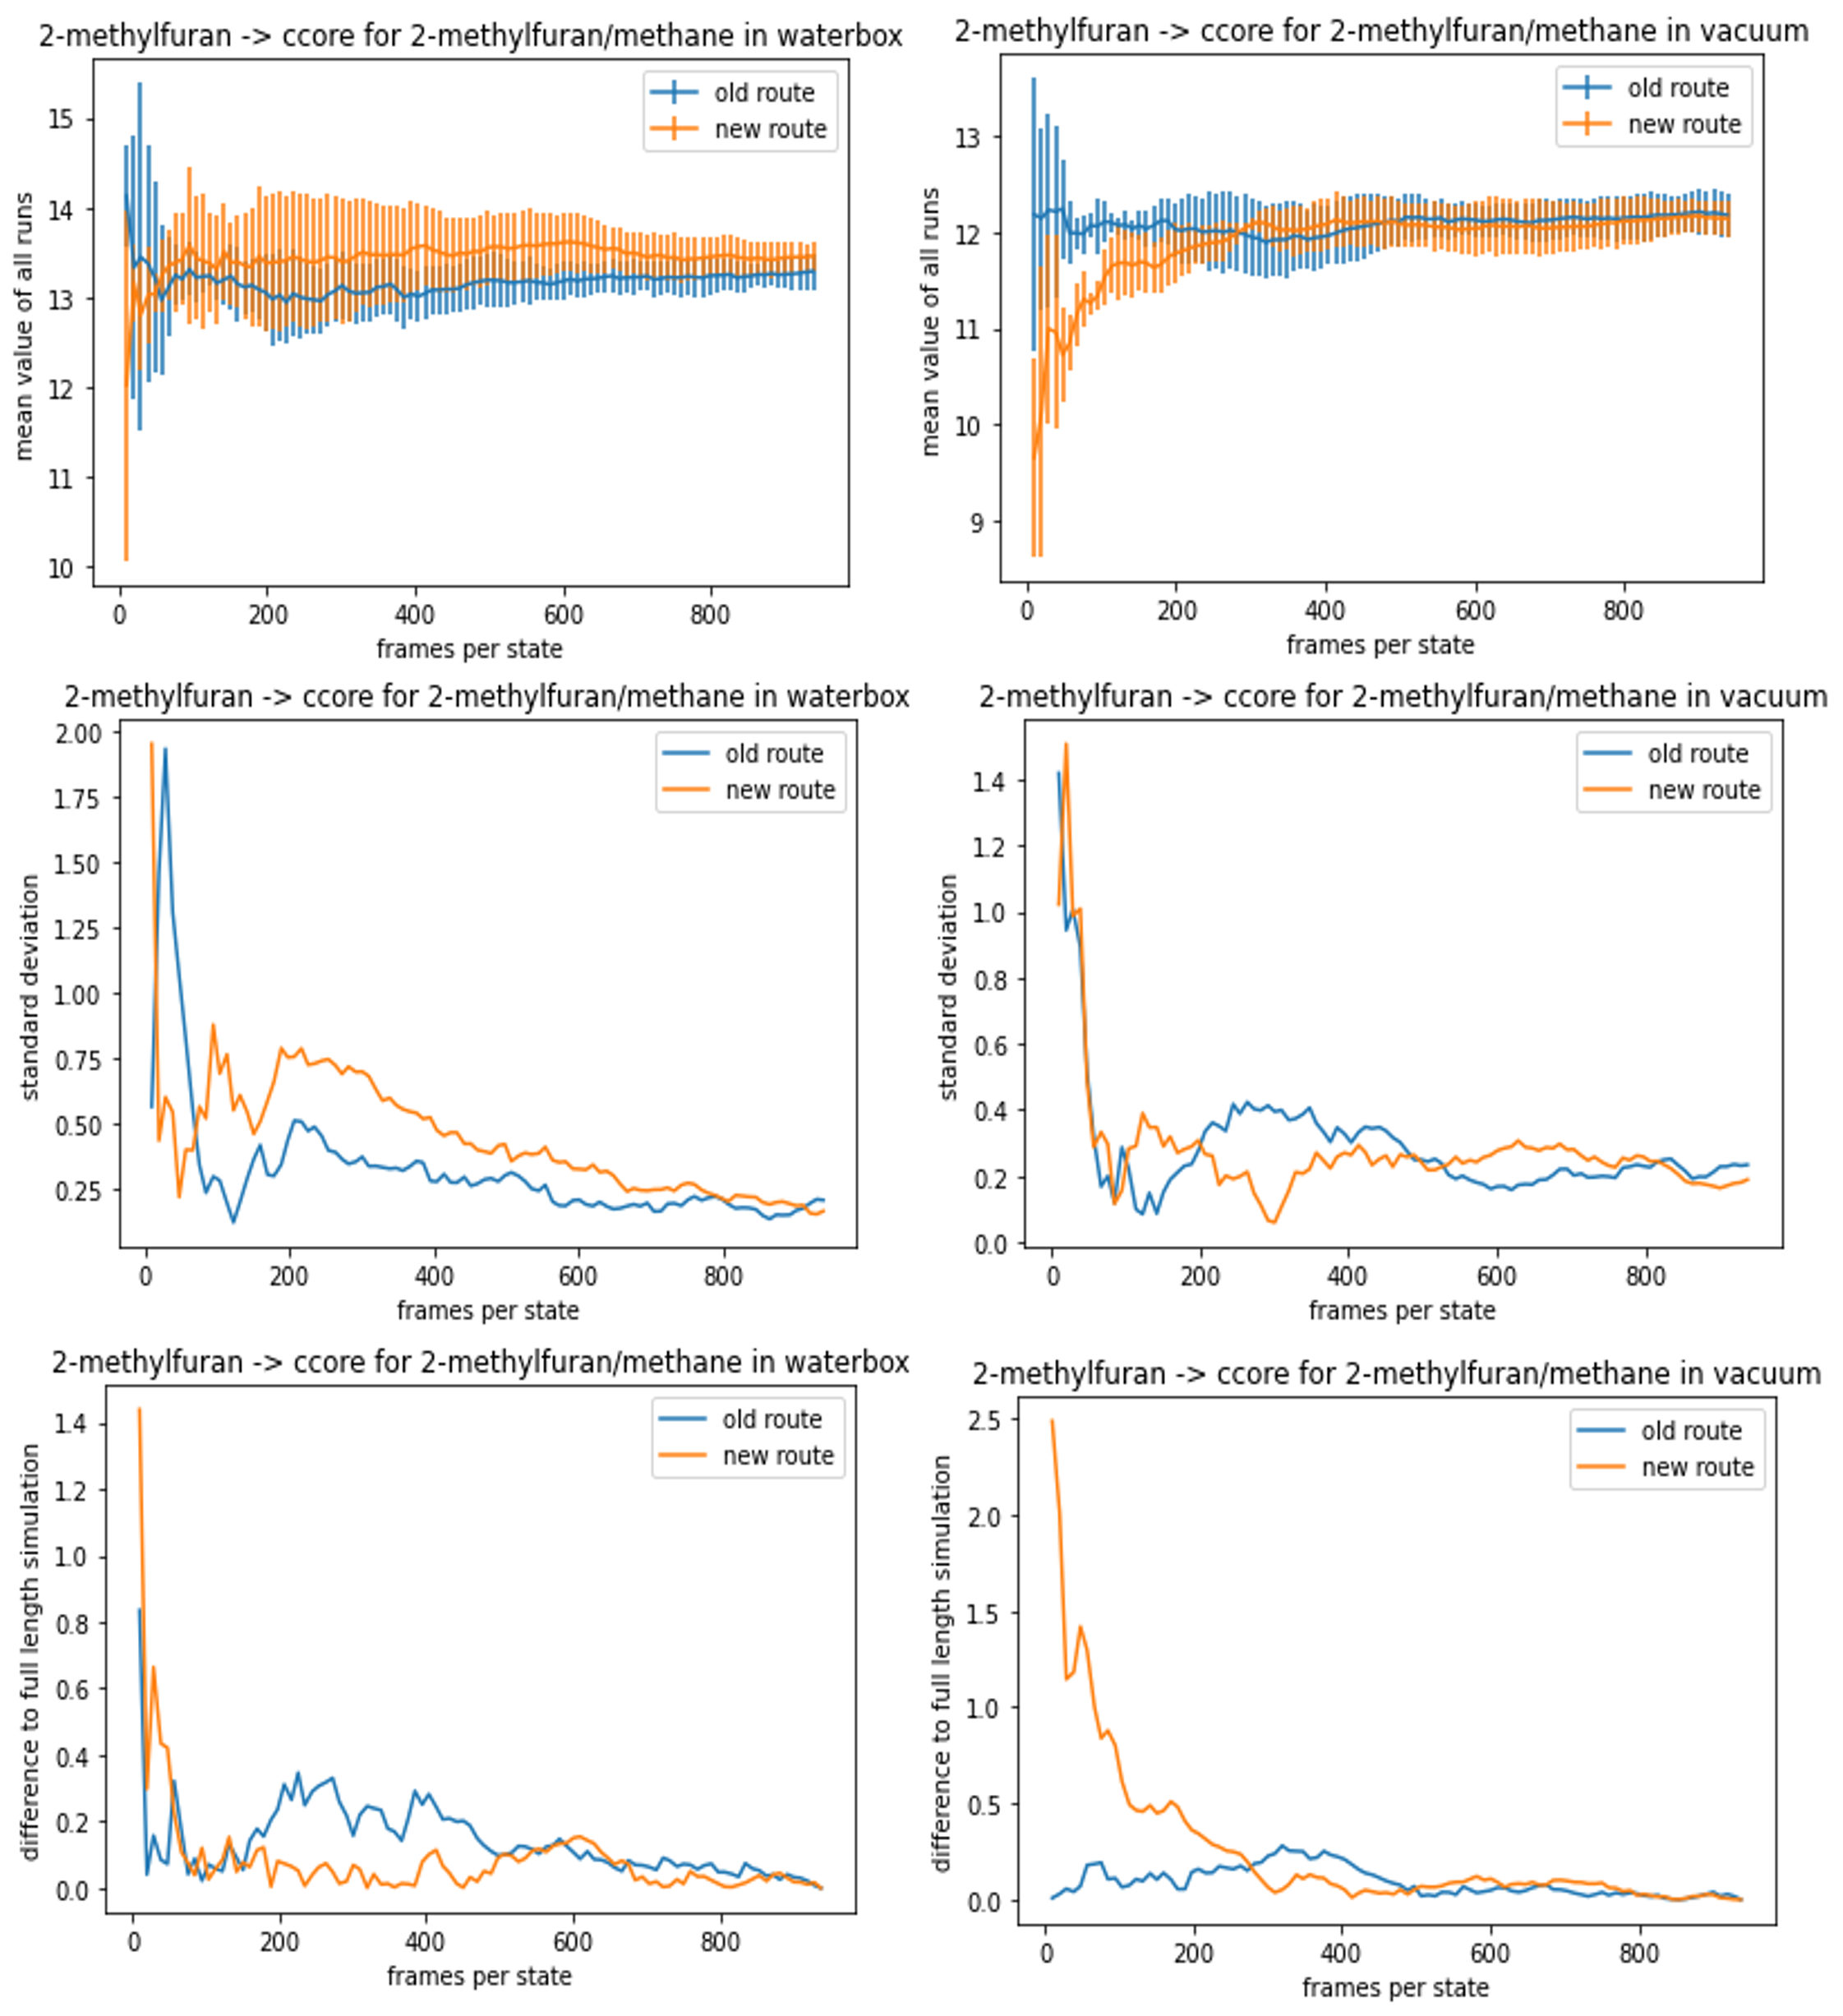
\includegraphics[scale=0.9]{methylfuran_short} \caption{2-methylfuran $\mathrm{\rightarrow}$ methane; left: water box; right: vacuum;  mutation routes for 2-methylfuran/methane; first row: mean value, bars indicate standard deviation; middle row: standard deviation; third row: difference to full-length simulation (i.e., the last value is zero)}
	\label{fig:methylfuran_short}
\end{figure}


\begin{figure}[!htb]
	
	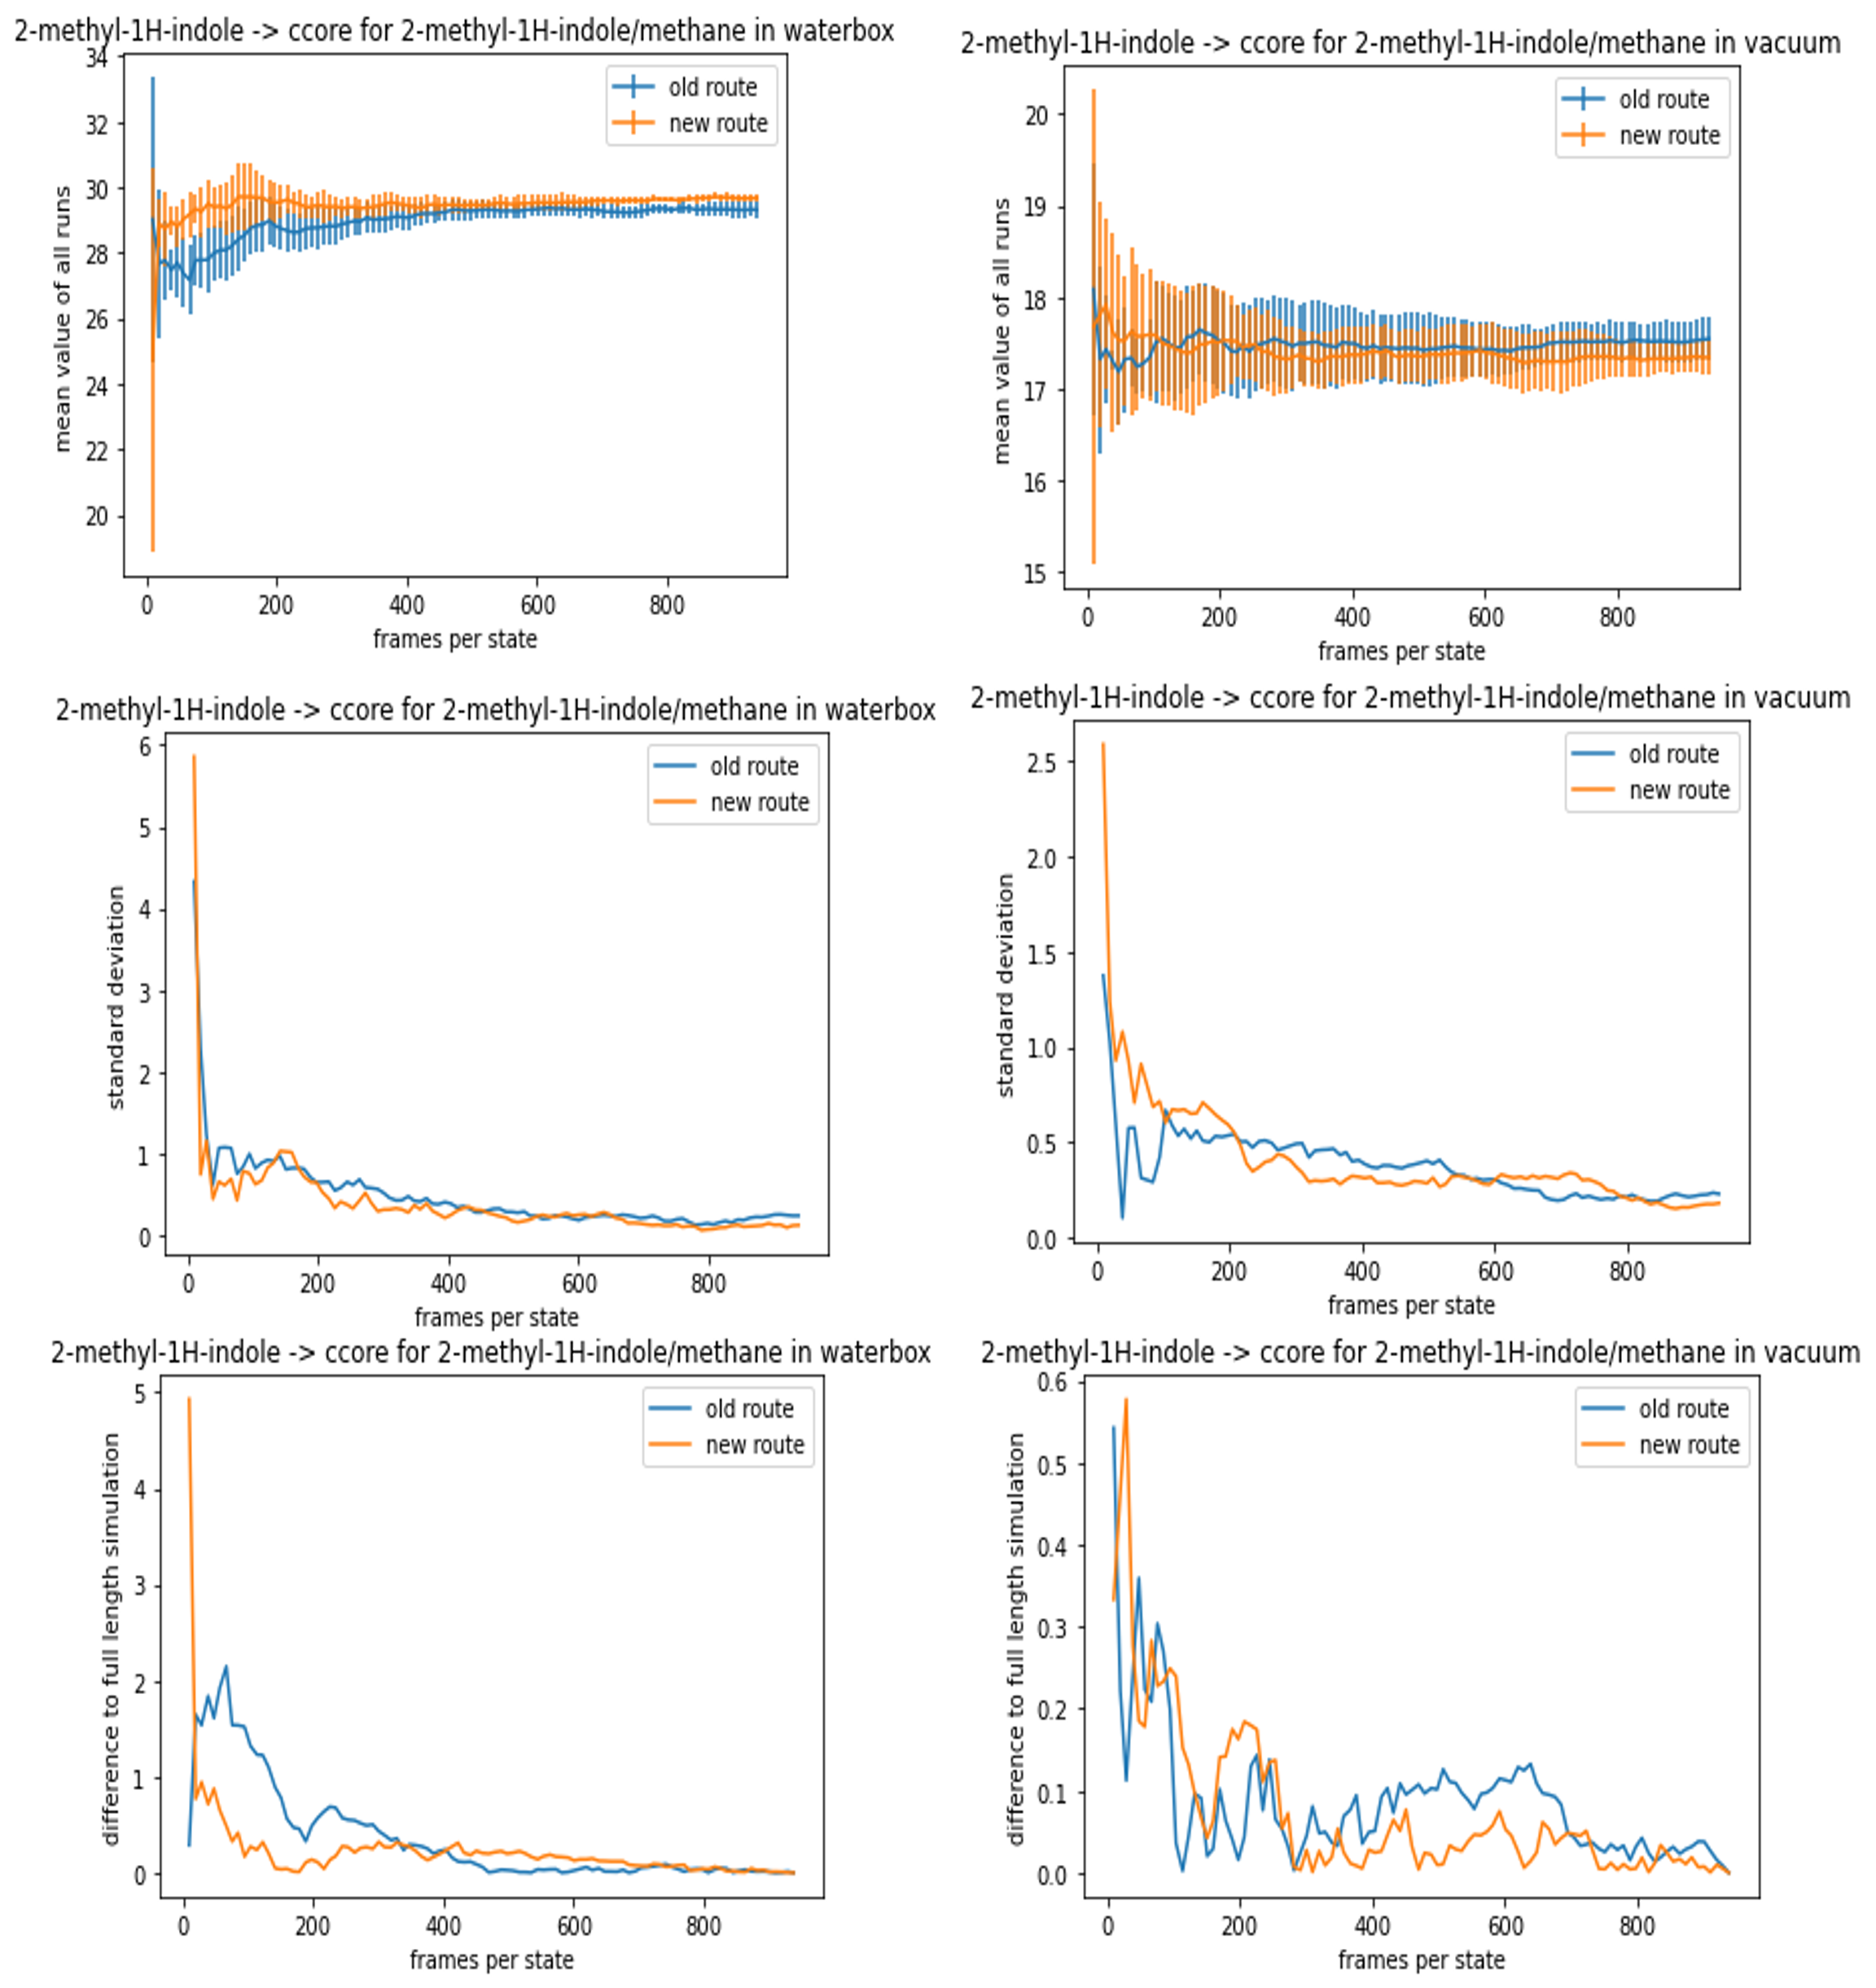
\includegraphics[scale=0.9]{methylindole_short}\caption{2-methylindole $\mathrm{\rightarrow}$ methane; left: water box; right: vacuum; mutation routes for 2-methylindole/methane; first row: mean value, bars indicate standard deviation; middle row: standard deviation; third row: difference to full-length simulation (i.e., the last value is zero)}
	\label{fig:methylindole_short}
\end{figure}

\begin{figure}[!htb]
	
	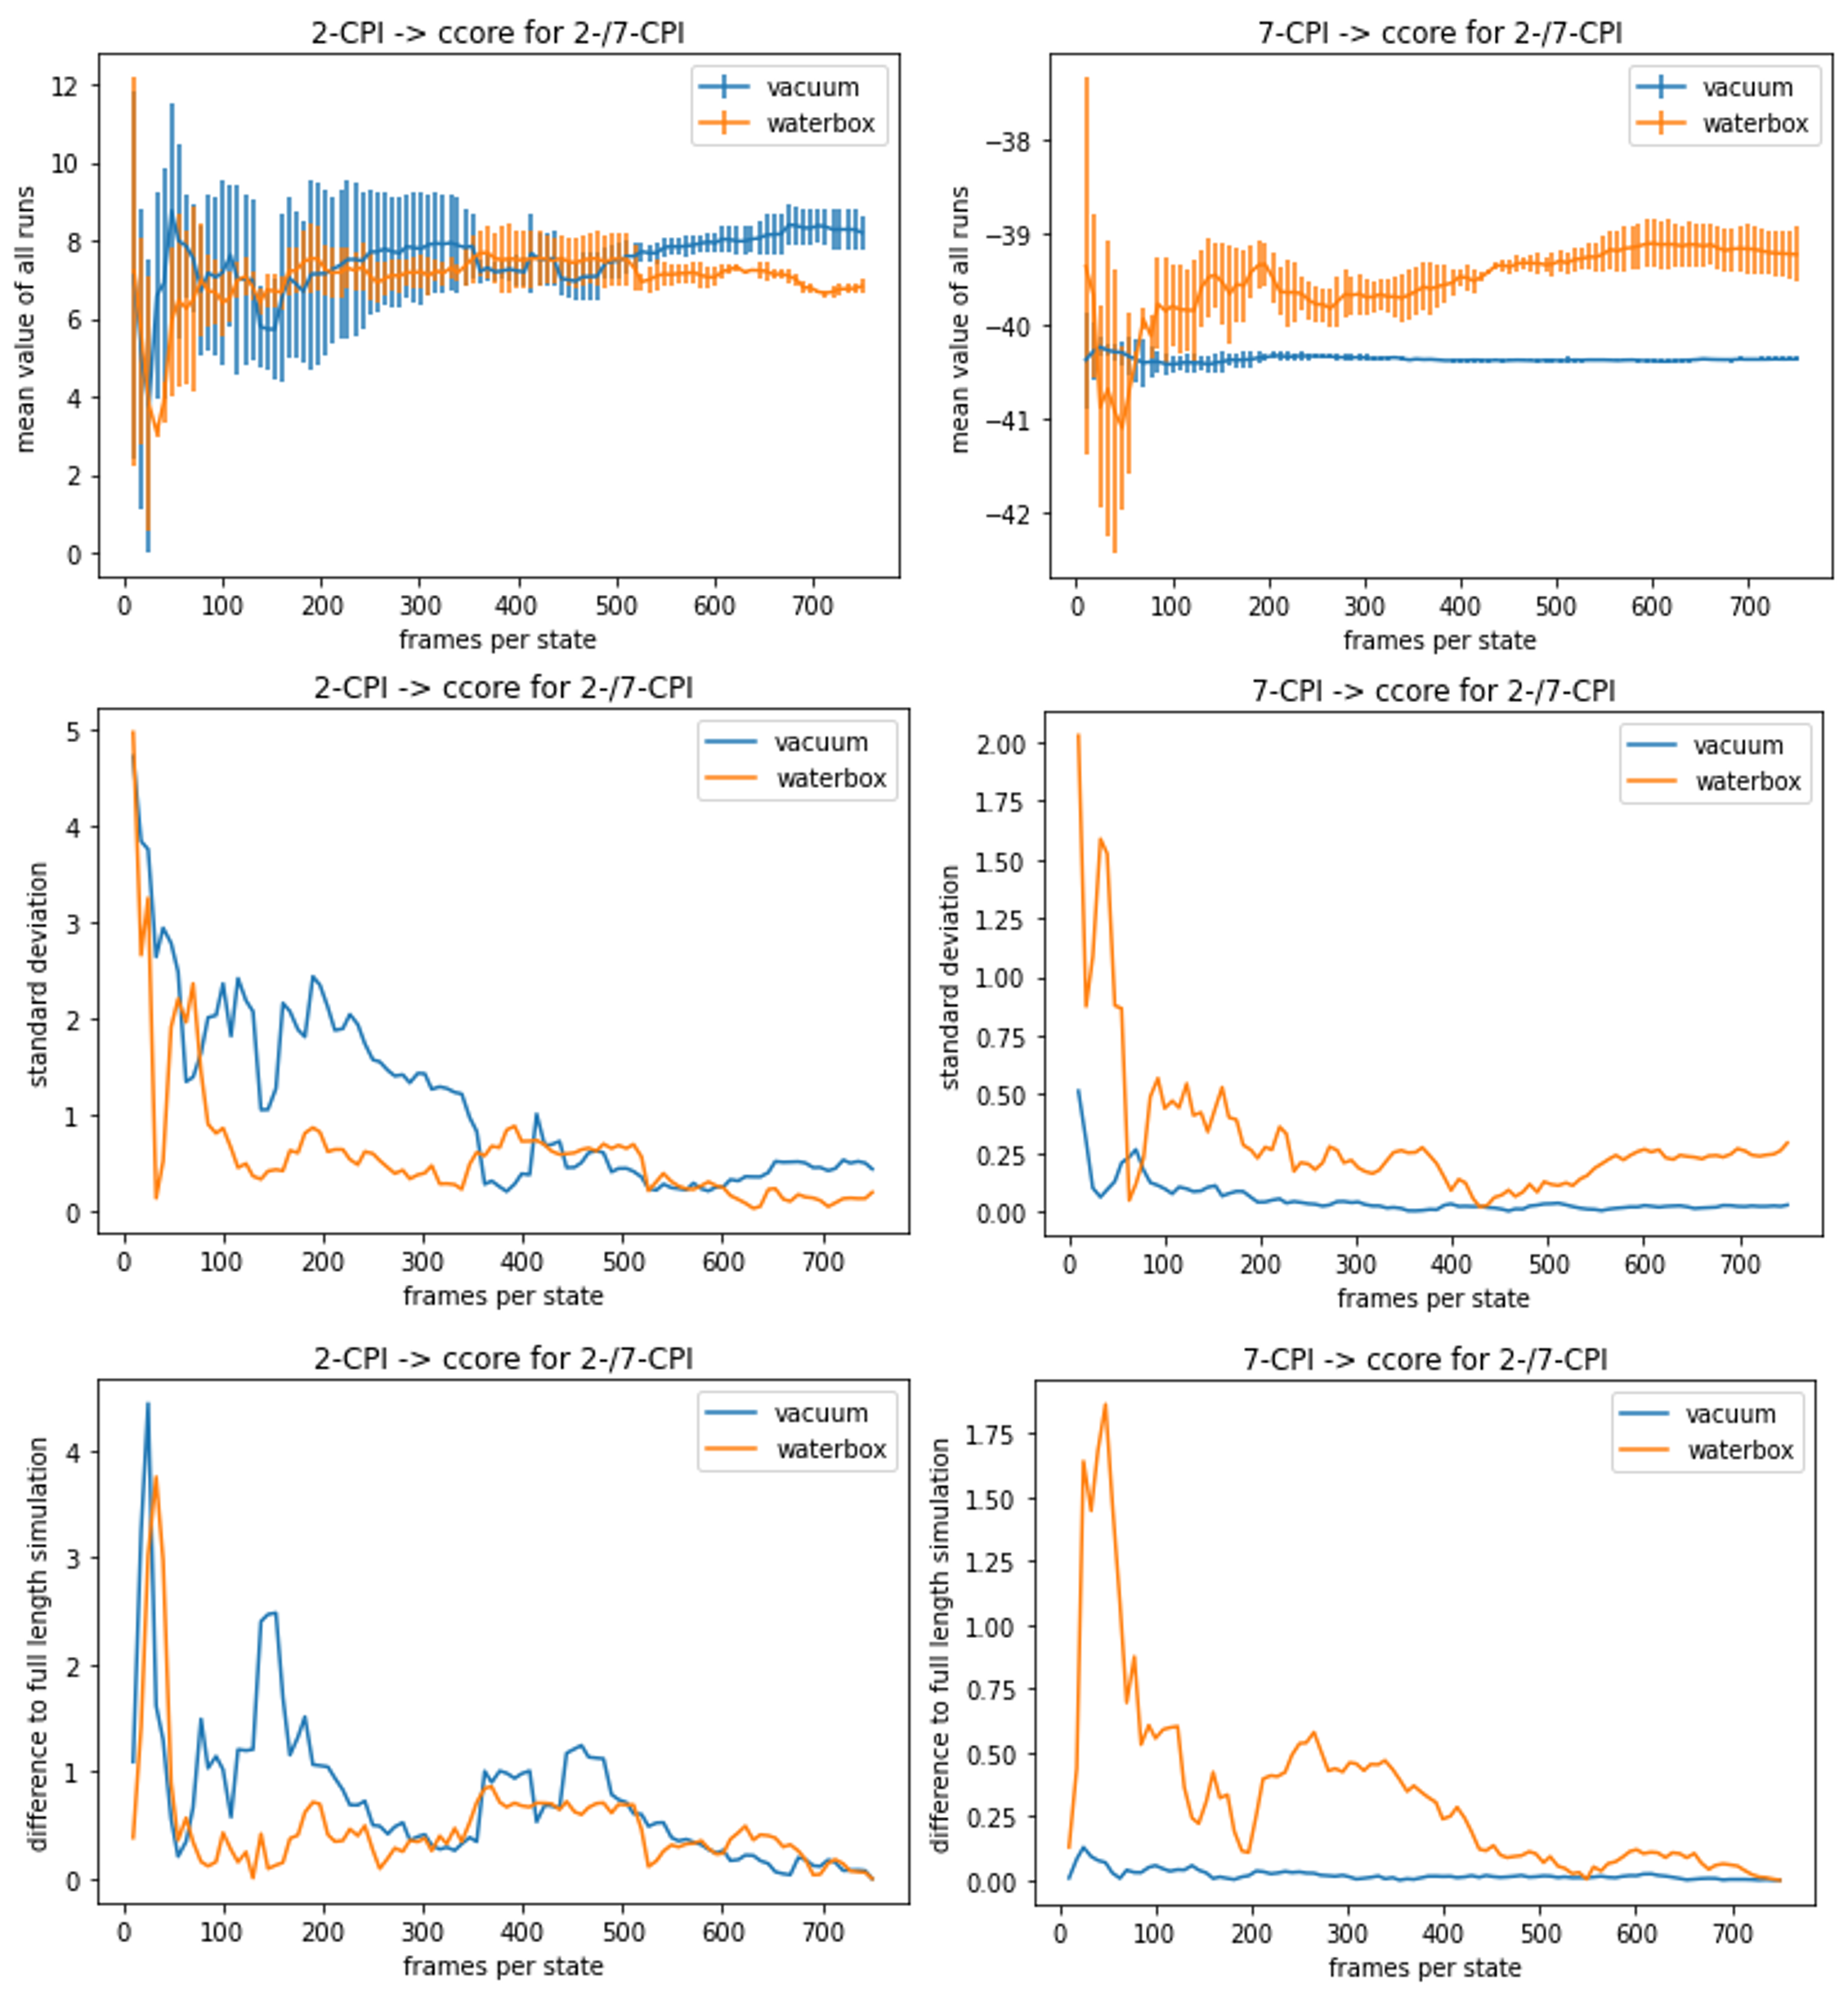
\includegraphics[scale=0.9]{cpi_short}\caption{left: 2-CPI $\mathrm{\rightarrow}$ CC for 2-/7-CPI; left: 7-CPI $\mathrm{\rightarrow}$ CC for 2-/7-CPI; first row: mean value, bars indicate standard deviation; middle row: standard deviation; third row: difference to full-length simulation (i.e., the last value is zero)}
	\label{fig:cpi_short}
\end{figure}
